%====================================================
% UNIVERSITY OF ECONOMICS HO CHI MINH CITY (UEH)
% GRADUATE ACADEMIC TEMPLATE 
%====================================================

\documentclass[12pt,a4paper]{article}

%----------------------------------------------------
% COLOR THEME (UEH)
%----------------------------------------------------
\usepackage{xcolor}
\definecolor{uehblue}{RGB}{0,70,127}
\definecolor{uehgray}{RGB}{80,80,80}

%----------------------------------------------------
% LANGUAGE & FONT
%----------------------------------------------------
\usepackage{polyglossia}
\usepackage{fontspec}
\setmainfont{Times New Roman}

%----------------------------------------------------
% PAGE LAYOUT
%----------------------------------------------------
\usepackage{geometry}
\geometry{
	left=3cm,
	right=2.5cm,
	top=3cm,
	bottom=3cm
}

\usepackage{setspace}
\onehalfspacing

\setlength{\parindent}{0pt}
\setlength{\parskip}{6pt}

% FIX HEADER HEIGHT
\setlength{\headheight}{14pt}

%----------------------------------------------------
% CORE PACKAGES
%----------------------------------------------------
\usepackage{graphicx}
\graphicspath{{figures/}}
\usepackage{booktabs}
\usepackage{longtable}
\usepackage{amsmath,amssymb}
%\usepackage{csquotes}
\usepackage{array}

\usepackage{graphicx}
\usepackage{subcaption}
\usepackage{float}
\usepackage{booktabs}
\usepackage{threeparttable}

\usepackage{tocloft}
\usepackage{etoolbox}

\usepackage{afterpage}

%----------------------------------------------------
% FIGURE & TABLE CAPTION
%----------------------------------------------------
\usepackage{caption}
\captionsetup{
	font=small,
	labelfont=bf,
	justification=raggedright,
	singlelinecheck=false
}

%----------------------------------------------------
% HYPERLINKS
%----------------------------------------------------
\usepackage{hyperref}
\hypersetup{
	colorlinks=true,
	linkcolor=black,
	citecolor=uehblue,
	urlcolor=blue
}

%----------------------------------------------------
% HEADER & FOOTER – UEH
%----------------------------------------------------
\usepackage{fancyhdr}
\usepackage{lastpage}
\pagestyle{fancy}
\fancyhf{}

% Header
\fancyhead[L]{\small\textit{Đại học Kinh tế Thành phố Hồ Chí Minh}}
\fancyhead[R]{\small\textit{Niên khóa 2025--2026}}

% Footer
\fancyfoot[L]{
\includegraphics[height=0.8cm]{logoueh.png}}
\fancyfoot[C]{\small\textit{Kinh tế sức khỏe}}
\fancyfoot[R]{\small Trang \thepage\ | \pageref{LastPage}}

\renewcommand{\headrulewidth}{0.4pt}
\renewcommand{\footrulewidth}{0pt}

%----------------------------------------------------
% SECTION FORMAT
%----------------------------------------------------
\usepackage{titlesec}
\titleformat{\section}{\bfseries\large}{\thesection.}{0.5em}{}
\titleformat{\subsection}{\bfseries}{\thesubsection}{0.5em}{}
\titleformat{\subsubsection}{\itshape}{\thesubsubsection}{0.5em}{}

%----------------------------------------------------
% BIBLIOGRAPHY – APA / HARVARD
%----------------------------------------------------
\usepackage[
backend=biber,
style=authoryear,
sorting=nyt,
maxcitenames=2,
maxbibnames=99,
doi=true,
url=true,
isbn=false
]{biblatex}

\addbibresource{references.bib}


%====================================================
% DOCUMENT START
%====================================================
\begin{document}
	
	%====================================================
	% TITLE PAGE – UEH
	%====================================================
	\begin{titlepage}
		\centering
{\large \textbf{BỘ GIÁO DỤC VÀ ĐÀO TẠO}}\\
{\Large \textbf{\textcolor{blue}{ĐẠI HỌC KINH TẾ THÀNH PHỐ HỒ CHÍ MINH}}}\\
\vspace{0.2cm}
\textbf{TRƯỜNG KINH TẾ, LUẬT VÀ QUẢN LÝ NHÀ NƯỚC}\\
\vspace{1.5cm}
		
		
\includegraphics[width=5cm]{logoueh.png}\\[1.2cm]
		
		{\large \textcolor{uehgray}{CHƯƠNG TRÌNH CAO HỌC}}\\[1.5cm]
		
		{\Huge \bfseries TÁC ĐỘNG CỦA BẢO HIỂM Y TẾ ĐẾN CHI TIÊU TIỀN TÚI CHO Y TẾ Ở KHU VỰC NÔNG THÔN VÀ THÀNH THỊ VIỆT NAM
		}\\[0.5 cm]
		{\large BÀI NGHIÊN CỨU NHÓM}\\[1 cm]
		
	\begin{flushleft}
		\textbf{Danh sách thành viên nhóm:}\\[0.5 cm]
		
		\begin{tabular}{ll}
			1. Trương Nhật Duy & MSSV: [ID redacted] \\
			2. Trần Ngọc Quân & MSSV: [ID redacted] \\
			3. Trần Phương Minh & MSSV: [ID redacted]\\
			4. Phạm Thị Thão Nguyên & MSSV: [ID redacted] \\
	
		\end{tabular}
		
		\vspace{0.5 cm}
		\textbf{Chuyên ngành:} Kinh tế Phát triển\\
		\textbf{Học phần:} Kinh tế sức khỏe\\

	\end{flushleft}
	\end{titlepage}
	
%====================================================
% TABLE OF CONTENTS
%====================================================

\makeatletter
% ẨN List of Figures
\renewcommand{\listoffigures}{%
	\@starttoc{lof}%          % Chỉ chạy danh sách, KHÔNG title
}
\renewcommand{\listfigurename}{}     % Để trống

% ẨN List of Tables  
\renewcommand{\listoftables}{%
	\@starttoc{lot}%          % Chỉ chạy danh sách, KHÔNG title
}
\renewcommand{\listtablename}{}      % Để trống

% ẨN Contents (nếu cần)
\renewcommand{\tableofcontents}{%
	\@starttoc{toc}%          % Chỉ chạy mục lục, KHÔNG title
}
\renewcommand{\contentsname}{}
\makeatother


% Mục lục
\section*{Mục lục}
\tableofcontents  
\newpage

% DANH MỤC HÌNH VẼ 
\section*{Danh mục hình vẽ}
\addcontentsline{toc}{section}{Danh mục hình vẽ}
\listoffigures   


% LIST OF TABLES  
\section*{Danh mục bảng biểu}
\addcontentsline{toc}{section}{Danh mục bảng biểu}
\listoftables
\newpage

\newpage
\section*{Danh mục các ký hiệu viết tắt}
\addcontentsline{toc}{section}{Danh mục các ký hiệu viết tắt}

\begin{table}[htbp]
	\centering
	\begin{tabular}{ll}
		\toprule
		\textbf{Viết tắt} & \textbf{Ý nghĩa} \\
		\midrule
		\textbf{Thuật ngữ chung} & \\
		BHYT & Bảo hiểm y tế \\
		OOP & Chi tiêu y tế từ tiền túi (\textit{Out-of-pocket expenditure}) \\
		UHC & Bao phủ y tế phổ quát (\textit{Universal Health Coverage}) \\
		VHLSS & Khảo sát mức sống dân cư Việt Nam (\textit{Vietnam Household Living Standard Survey}) \\
		WHO & Tổ chức Y tế Thế giới (\textit{World Health Organization}) \\
		SDG & Mục tiêu phát triển bền vững (\textit{Sustainable Development Goals}) \\
		OTC & Thuốc không kê đơn (\textit{Over-the-counter}) \\
		
		\addlinespace
		\textbf{Phương pháp luận} & \\
		IV-2SLS & Phương pháp biến công cụ hai giai đoạn (\textit{Instrumental Variables 2-Stage Least Squares}) \\
		SQREG & Hồi quy phân vị đồng thời (\textit{Simultaneous Quantile Regression}) \\
		PSM & Ghép cặp điểm xu hướng (\textit{Propensity Score Matching}) \\
		VIF & Hệ số phóng đại phương sai (\textit{Variance Inflation Factor}) \\
		ICC & Hệ số tương quan nội cụm (\textit{Intraclass Correlation Coefficient}) \\
		ATE & Tác động xử lý trung bình (\textit{Average Treatment Effect}) \\
		FE & Hiệu ứng cố định (\textit{Fixed Effects}) \\
		
		\addlinespace
		\textbf{Ký hiệu biến số} & \\
		\texttt{INS} & Biến giả hộ gia đình có tham gia Bảo hiểm y tế \\
		\texttt{RURAL} & Biến giả hộ gia đình sinh sống tại khu vực nông thôn \\
		\texttt{BYP / BYPASSED} & Biến giả hành vi khám chữa bệnh vượt tuyến/trái tuyến \\
		\texttt{INC / ln\_INC} & Thu nhập bình quân đầu người (dạng logarit) \\
		$OOP_{in}$ & Chi tiêu y tế cho điều trị nội trú \\
		$OOP_{out}$ & Chi tiêu y tế cho điều trị ngoại trú \\
		\bottomrule
	\end{tabular}
\end{table}

%====================================================
% MAIN CONTENT
%====================================================
\newpage
\section*{Tóm tắt}
\addcontentsline{toc}{section}{Tóm tắt}

Nghiên cứu này phân tích tác động nhân quả của Bảo hiểm y tế (BHYT) đối với chi tiêu y tế từ tiền túi (OOP) của hộ gia đình Việt Nam, với trọng tâm là nhận diện "hiệu ứng kép" của BHYT giữa các loại hình dịch vụ và vai trò điều tiết của hành vi vượt tuyến. Sử dụng dữ liệu từ Khảo sát Mức sống Dân cư Việt Nam (VHLSS) năm 2024, nghiên cứu áp dụng phối hợp các phương pháp kinh tế lượng tiên tiến bao gồm Biến công cụ (IV-2SLS), Hồi quy phân vị đồng thời (SQREG) và Ghép cặp điểm xu hướng (PSM) nhằm kiểm soát triệt để hiện tượng nội sinh và thiên lệch tự lựa chọn.

Kết quả thực nghiệm bác bỏ quan điểm đơn giản cho rằng BHYT luôn làm giảm gánh nặng tài chính. Thay vào đó, nghiên cứu xác nhận sự tồn tại của một \textbf{"hiệu ứng kép"} phi tuyến: (i) BHYT làm tăng tổng chi phí OOP và chi phí ngoại trú, phản ánh việc khơi thông nhu cầu y tế bị kìm nén nhưng cũng hàm ý sự xuất hiện của rủi ro đạo đức (moral hazard); (ii) Ngược lại, đối với các rủi ro y tế thảm họa, BHYT vận hành như một lưới an sinh vững chắc. Đặc biệt, khi bệnh nhân nông thôn buộc phải vượt tuyến điều trị nội trú, BHYT giúp giảm đáng kể chi phí thực tế. Kết quả từ mô hình SQREG cho thấy "hình phạt tài chính" của hành vi vượt tuyến tăng đột biến lên mức $2,039$ tại phân vị 90 ($Q90$), và chính tại ngưỡng thảm họa này, năng lực bảo vệ tài chính của BHYT được phát huy mạnh mẽ nhất (hệ số $-0,605$).

Nghiên cứu đóng góp vào kho tàng thực nghiệm theo ba hướng: thứ nhất, minh chứng tính phi tuyến của BHYT thông qua việc phân tách cấu trúc chi phí nội-ngoại trú; thứ hai, lượng hóa sự biến thiên của chi phí vượt tuyến dọc theo phân phối OOP; và thứ ba, cung cấp bằng chứng nhân quả cập nhật nhất từ bối cảnh Việt Nam năm 2024. 

Về mặt hàm ý, nghiên cứu nhấn mạnh lộ trình đạt tới Bao phủ y tế phổ quát (UHC) cần chuyển dịch trọng tâm từ mở rộng diện bao phủ hình thức sang tăng cường "độ sâu" quyền lợi. Các giải pháp bao gồm: mở rộng danh mục thuốc ngoại trú tại y tế cơ sở nông thôn, đổi mới cơ chế thanh toán và áp dụng đồng chi trả thông minh nhằm tối ưu hóa hành vi sử dụng dịch vụ của người dân.

\vspace{0.5em}
\noindent \textbf{Từ khóa:} Bảo hiểm y tế; Chi tiêu tiền túi (OOP); Hiệu ứng kép; IV-2SLS; SQREG; Hành vi vượt tuyến; Kinh tế y tế.

\newpage
\section{Giới thiệu}

Việt Nam đã đạt được những thành tựu mang tính bước ngoặt trong nỗ lực mở rộng độ bao phủ Bảo hiểm y tế (BHYT). Tính đến năm 2024, tỷ lệ bao phủ toàn dân đã vượt ngưỡng 92,1\%, tiệm cận mục tiêu của Nghị quyết 20-NQ/TW về bảo vệ và chăm sóc sức khỏe nhân dân \parencite{gso2024}. Những bước tiến về khung pháp lý, đặc biệt là Luật BHYT sửa đổi, đã đánh dấu sự chuyển đổi mạnh mẽ từ mô hình bảo hiểm tự nguyện sang bảo hiểm bắt buộc, đặt nền móng vững chắc cho tiến trình Bao phủ Y tế Phổ quát (UHC).

Tuy nhiên, đằng sau sự gia tăng ấn tượng về độ bao phủ, hệ thống y tế vẫn đang đối mặt với một nghịch lý lớn: Gánh nặng chi phí y tế từ tiền túi (OOP) vẫn duy trì ở mức cao. Theo báo cáo của Ngân hàng Thế giới (2024), chi tiêu OOP chiếm khoảng 41,3\% tổng chi tiêu y tế quốc gia, vượt xa ngưỡng an toàn 30--35\% do Tổ chức Y tế Thế giới (WHO) khuyến cáo \parencite{who2023}. Đáng quan ngại hơn, tình trạng chi tiêu y tế thảm họa vẫn liên tục đe dọa các hộ gia đình yếu thế, với tỷ lệ mắc phải tại khu vực nông thôn thường cao gấp đôi so với thành thị \parencite{gso2024}, tạo ra rào cản lớn trong việc hiện thực hóa công bằng y tế.

\subsection{Vấn đề nghiên cứu then chốt}

Sự tồn tại dai dẳng của gánh nặng OOP, bất chấp tỷ lệ bao phủ BHYT tiệm cận mức tuyệt đối, làm nảy sinh câu hỏi về hiệu quả thực chất của chính sách BHYT. Nghịch lý này bắt nguồn từ những đặc điểm cấu trúc phức tạp và sự phân hóa về địa lý trong y tế tại Việt Nam:

\begin{itemize}
	\item \textbf{Tại khu vực Nông thôn:} Do hạn chế về hạ tầng y tế cơ sở và danh mục thuốc chi trả hẹp, người dân thường có xu hướng tự điều trị bằng thuốc không kê đơn (OTC), dẫn đến việc phải tự chi trả 100\% OOP cho các dịch vụ ngoại trú \parencite{lee2019ijerph}. Tuy nhiên, khi đối mặt với bệnh lý nặng, họ phải chịu áp lực tài chính kép từ chi phí di chuyển và hình phạt tài chính (financial penalty) khổng lồ do hành vi khám chữa bệnh vượt tuyến.
	
	\item \textbf{Tại khu vực Thành thị:} Sự tập trung của các bệnh viện tuyến cuối tạo điều kiện thuận lợi cho việc tiếp cận dịch vụ kỹ thuật cao. Tại đây, BHYT dễ dàng kích hoạt rủi ro đạo đức (moral hazard) từ cả phía cung và phía cầu, làm gia tăng tần suất sử dụng dịch vụ ngoại trú và các loại thuốc ngoài danh mục, gián tiếp đẩy tổng mức chi tiêu OOP lên cao \parencite{thuong2020did}.
\end{itemize}

Thực trạng này đặt ra câu hỏi nghiên cứu trung tâm rằng: Liệu BHYT đang đóng vai trò là một lá chắn tài chính vững chắc trước các cú sốc bệnh tật thảm họa hay chỉ đơn thuần là chất xúc tác làm gia tăng chi phí y tế ?

\subsection{Mục tiêu và đóng góp nghiên cứu}

Để giải quyết bài toán trên, nghiên cứu này áp dụng môt hệ thống phương pháp định lượng đồng bộ, bao gồm: Mô hình Biến công cụ (IV-2SLS), Hồi quy phân vị đồng thời (SQREG) và Ghép cặp điểm xu hướng (PSM) trên bộ dữ liệu Khảo sát Mức sống Dân cư Việt Nam (VHLSS) năm 2024 ($N = 46.995$). Nghiên cứu tập trung trả lời ba câu hỏi cốt lõi:

\begin{enumerate}
	\item \textbf{Nhận diện Hiệu ứng kép của BHYT:} Sau khi kiểm soát triệt để vấn đề nội sinh, tác động thực sự của BHYT lên cấu trúc chi phí (chi phínội trú thảm họa so với chi phí ngoại trú thường nhật) diễn ra theo cơ chế nào?
	
	\item \textbf{Cơ chế điều tiết của hành vi vượt tuyến:} Hành vi tự ý vượt tuyến định hình lại gánh nặng OOP ra sao dọc theo phân phối chi phí? BHYT phát huy năng lực bảo vệ tài chính mạnh nhất tại phân vị nào?
	
	\item \textbf{Định hướng chính sách:} Dựa trên bằng chứng thực nghiệm và đối chiếu với kinh nghiệm quốc tế \parencite{feldstein2011}, làm thế nào để chuyển dịch từ bao phủ hình thức sang tăng cường độ sâu quyền lợi chi trả?
\end{enumerate}

Nghiên cứu mang lại ba đóng góp mới về mặt học thuật và thực tiễn: (i) Lần đầu tiên phân tách chi tiết cấu trúc OOP để lượng hóa tính phi tuyến của BHYT thông qua "Hiệu ứng kép"; (ii) Lượng hóa sự leo thang của chi phí vượt tuyến thông qua lăng kính hồi quy phân vị, giúp nhận diện chính xác ngưỡng thảm họa; và (iii) Cung cấp bằng chứng nhân quả cập nhật nhất từ dữ liệu quy mô lớn VHLSS 2024, đóng góp tiếng nói thực nghiệm quan trọng vào tiến trình thực hiện Mục tiêu Phát triển Bền vững (SDG 3.8) tại Việt Nam.

\section{Cơ sở lý thuyết và tổng quan tài liệu}

Nghiên cứu xây dựng khung phân tích dựa trên sự tổng hợp lý thuyết kinh tế học y tế của \textcite{folland2024} và mô hình chi phí thời gian của \textcite{sarkodie2022}, đặt trong bối cảnh mô hình vốn sức khỏe tổng quát của \textcite{grossman1972}. Theo đó, cơ chế tác động của Bảo hiểm Y tế (BHYT) đến hành vi tiêu dùng dịch vụ và chi tiêu tiền túi (OOP) được diễn giải thông qua hai kênh truyền dẫn chính: (i) Kênh giá tài chính và (ii) Kênh chi phí thời gian.

\subsection{Cơ chế đồng chi trả, Rủi ro đạo đức và Độ co giãn của cầu}

Theo \textcite{folland2024}, cầu đối với dịch vụ y tế chịu sự bóp méo mạnh mẽ bởi cơ chế bảo hiểm. Trong điều kiện không có bảo hiểm, cá nhân đối mặt với giá thị trường toàn phần ($P_M$). Khi có BHYT, thông qua tỷ lệ đồng chi trả ($r$, với $0 < r < 1$), giá thực tế tại thời điểm sử dụng dịch vụ (\textit{effective out-of-pocket price}) giảm xuống còn $rP_M$.

\begin{figure}[ht]
	
	\centering
	
	\includegraphics[width=0.8\textwidth]{lythuyetcungcauFolland.bmp}
	
	\caption{Tác động của tỷ lệ đồng chi trả đến cầu chăm sóc sức khỏe}
	
	\par\small\textit{Nguồn: \textcite{folland2024}}
	
	\label{fig:folland_demand}
	
\end{figure}

Sự sụt giảm giá biên này tạo ra hiệu ứng thay thế, làm dịch chuyển lượng cầu từ $Q_0$ lên $Q_1$ như minh họa trong lý thuyết của \textcite{folland2024}. Tuy nhiên, \textcite{arrow1963} nhấn mạnh rằng sự chênh lệch giữa chi phí biên xã hội và chi phí biên cá nhân kích hoạt hiện tượng \textbf{rủi ro đạo đức (moral hazard)}. Do không gánh chịu toàn bộ chi phí, người bệnh có xu hướng gia tăng sử dụng các dịch vụ ngoại trú, thuốc men hoặc xét nghiệm vượt mức cần thiết. Hệ quả là, BHYT có thể dẫn đến sự gia tăng tổng chi tiêu OOP thay vì cắt giảm như kỳ vọng ban đầu.

\subsection{Vai trò điều tiết của Giá thời gian và Khác biệt không gian}

Dựa trên khung phân tích của \textcite{sarkodie2022}, tổng chi phí thực tế (\textit{Full Price} - $\pi$) mà người bệnh gánh chịu bao gồm cả chi phí tiền mặt và chi phí cơ hội của thời gian:

\begin{equation}
	\pi_{ij} = \underbrace{r \cdot P_{M}}_{\text{Chi phí tài chính (OOP)}} + \underbrace{w_i \cdot (T_{\text{travel}} + T_{\text{wait}})}_{\text{Chi phí thời gian}}
\end{equation}

Trong đó, $w_i$ là chi phí cơ hội của thời gian; $T_{\text{travel}}$ và $T_{\text{wait}}$ là thời gian di chuyển và chờ đợi. Mô hình này cho thấy sự phân hóa cấu trúc giữa hai khu vực:
\begin{enumerate}
	\item \textbf{Tại thành thị:} $T_{\text{travel}}$ thấp khiến tổng chi phí $\pi$ bị chi phối bởi $rP_M$. BHYT dễ dàng kích hoạt rủi ro đạo đức, đẩy cao tần suất khám ngoại trú và các chi phí thuốc ngoài danh mục.
	\item \textbf{Tại nông thôn:} Mặc dù $rP_M$ giảm, nhưng $T_{\text{travel}}$ lớn là rào cản chủ đạo. Với bệnh nhẹ, người dân ưu tiên tự điều trị để tiết kiệm thời gian. Tuy nhiên, khi mắc bạo bệnh buộc phải vượt tuyến, BHYT chuyển trạng thái từ công cụ kích cầu sang "lưới an sinh" nhằm hấp thụ các cú sốc tài chính thảm họa.
\end{enumerate}

\subsection{Tổng quan nghiên cứu thực nghiệm}

Các bằng chứng thực nghiệm tại Việt Nam ghi nhận những kết quả không đồng nhất, phản ánh sự chuyển đổi mô hình chính sách qua các thời kỳ (Bảng \ref{tab:litreview}).

\begin{table}[htbp]
	\centering
	\small
	\caption{Tổng hợp các nghiên cứu thực nghiệm tiêu biểu tại Việt Nam}
	\label{tab:litreview}
	\begin{tabular}{p{2.5cm}p{2.2cm}p{2.2cm}p{4cm}p{3cm}}
		\toprule
		\textbf{Nghiên cứu} & \textbf{Dữ liệu} & \textbf{Phương pháp} & \textbf{Kết quả chính} & \textbf{Hạn chế} \\
		\midrule
		\textcite{jowett2003} & VLSS 1998 & OLS & Giảm OOP từ 15--20\% & Nội sinh chưa xử lý \\
		\textcite{thuong2020did} & VHLSS 2014-16 & DID & Tăng lượt khám ngoại trú & Chưa xét vượt tuyến \\
		\textcite{lee2019ijerph} & VHLSS 2016 & Tobit & Giảm OOP nông thôn $\sim$12\% & Thiếu đánh giá phi tuyến \\
		\textcite{giang2022} & VHLSS 2020 & PSM & BHYT chưa giảm sốc tài chính & Chệch do biến ẩn \\
		\bottomrule
	\end{tabular}
\end{table}

Các nghiên cứu gần đây như \textcite{thuong2020bmj} chỉ ra rằng BHYT có thể làm gia tăng sử dụng dịch vụ y tế chính thức, dẫn đến chi phí phát sinh tăng thêm. Điều này củng cố giả thuyết về "hiệu ứng kép" mà nghiên cứu này hướng tới.

\subsection{Khoảng trống học thuật và đóng góp của nghiên cứu}

Các nghiên cứu hiện tại vẫn bộc lộ ba khoảng trống nền tảng mà nghiên cứu này tập trung lấp đầy:

\begin{itemize}
	\item \textbf{Xử lý nội sinh:} Thay vì các phương pháp truyền thống, nghiên cứu sử dụng Biến công cụ (IV) cấp xã để giải quyết triệt để hiện tượng tự lựa chọn.
	\item \textbf{Phân rã cấu trúc chi phí:} Bóc tách OOP thành nội trú (thảm họa) và ngoại trú (rủi ro đạo đức) để nhận diện tính chất đối lập trong tác động của BHYT.
	\item \textbf{Lượng hóa tính phi tuyến:} Sử dụng hồi quy phân vị (SQREG) để đo lường mức độ bảo vệ tài chính tại "đỉnh rủi ro" ($Q90$), nơi các mô hình hồi quy trung bình thường bỏ qua.
\end{itemize}

\section{Phương pháp nghiên cứu}
\subsection{Chiến lược ước lượng}

Để giải quyết triệt để vấn đề nội sinh, hiện tượng tự lựa chọn (self-selection bias) và kiểm tra tính vững của các kết quả ước lượng, nghiên cứu này áp dụng chiến lược kết hợp ba phương pháp bổ trợ:

\textbf{1. Phương pháp Biến công cụ hai giai đoạn (IV-2SLS)}

Đây là phương pháp chủ đạo nhằm xử lý triệt để vấn đề nội sinh của biến BHYT ($\text{INS}_i$), vốn thường phát sinh từ hiện tượng tự lựa chọn (self-selection) hoặc các đặc điểm không quan sát được liên quan đến tình trạng sức khỏe của hộ gia đình. Nghiên cứu sử dụng biến công cụ ($Z_i$) là tỷ lệ bao phủ BHYT bình quân cấp xã, được tính theo phương pháp loại trừ chính hộ gia đình đang quan sát (\textit{leave-one-out mean}):
\begin{equation}
	Z_i = \frac{1}{N_{c}-1} \sum_{j \neq i}^{N_{c}} INS_{j}
\end{equation}
Trong đó $N_c$ là tổng số hộ trong xã $c$. Việc lựa chọn biến công cụ này được bảo chứng bởi các cơ sở lý luận và thực nghiệm quan trọng:

\begin{itemize}
	\item \textit{Tính phù hợp (Instrument Relevance):} Cơ sở của biến công cụ này dựa trên lý thuyết về \textbf{hiệu ứng đồng cấp (peer effects)} và tương tác xã hội trong kinh tế học hành vi \parencite{manski1993}. Tại các cộng đồng có tỷ lệ bao phủ cao, chi phí tìm kiếm thông tin về quyền lợi và thủ tục BHYT của hộ gia đình giảm đáng kể. Đồng thời, áp lực từ các chuẩn mực xã hội địa phương thúc đẩy các hộ gia đình tham gia bảo hiểm để đảm bảo an sinh tương đồng với cộng đồng xung quanh. Cách tiếp cận này kế thừa từ nghiên cứu kinh điển của \textcite{wagstaff2007} về tác động của BHYT tại Việt Nam.
	
	\item \textit{Giả định loại trừ (Exclusion Restriction):} Bằng kỹ thuật \textit{leave-one-out}, nghiên cứu triệt tiêu hiện tượng "phản xạ" (reflection problem), đảm bảo $Z_i$ hoàn toàn ngoại sinh với sai số của hộ gia đình $i$. Tỷ lệ bao phủ chung của xã phản ánh năng lực vận động của chính quyền địa phương và môi trường thông tin đặc thù của khu vực, vốn không tác động trực tiếp đến chi tiêu OOP của cá nhân trừ khi thông qua kênh tham gia BHYT. Nghiên cứu cũng kiểm soát thêm Hiệu ứng cố định cấp tỉnh ($\delta_p$) để loại bỏ các yếu tố gây nhiễu liên quan đến chất lượng hạ tầng y tế vùng miền.
\end{itemize}

Mô hình cấu trúc giai đoạn hai (Second-stage) được thiết lập với các biến tương tác nhằm bóc tách tác động dị biệt:
\begin{equation}
	\ln(OOP_i + 1) = \alpha + \beta_1 \widehat{INS}_i + \beta_2 (\widehat{INS}_i \times RURAL_i) + \beta_3 (\widehat{INS}_i \times RURAL_i \times BYP_i) + \gamma X_i + \delta_p + \epsilon_i
\end{equation}
Trong đó, $\widehat{INS}_i$ là giá trị dự báo được ước lượng từ phương trình giai đoạn một (First-stage):
\begin{equation}
	INS_i = \pi_0 + \pi_1 Z_i + \pi_2 X_i + \delta_p + \nu_i
\end{equation}
Việc tích hợp biến tương tác vào mô hình IV đòi hỏi phải công cụ hóa tương ứng các cụm tương tác để đảm bảo các ước lượng $\beta_1, \beta_2, \beta_3$ là không chệch và nhất quán.

\textbf{2. Hồi quy Phân vị Đồng thời (Simultaneous Quantile Regression - SQREG)}

Để vượt qua giới hạn của hồi quy OLS vốn chỉ tập trung vào giá trị trung bình, nghiên cứu sử dụng phương pháp SQREG do \textcite{koenker1978} khởi xướng. Lựa chọn này dựa trên các cơ sở học thuật quan trọng:
\begin{itemize}
	\item \textit{Tính không đồng nhất (Heterogeneity):} Trong kinh tế học y tế, tác động của BHYT thường không đồng nhất dọc theo phân phối chi phí. \textcite{bitler2006} lập luận rằng việc chỉ tập trung vào tác động trung bình có thể che lấp các hiệu ứng quan trọng tại các nhóm yếu thế. SQREG cho phép lượng hóa tác động của BHYT tại nhóm gánh chịu chi phí thảm họa ($Q90$) — nơi mà năng lực bảo vệ tài chính của bảo hiểm là cấp thiết nhất.
	\item \textit{Tính vững đối với giá trị ngoại lai:} Dữ liệu chi tiêu y tế thường có đuôi dài (heavy-tailed) và nhiều giá trị ngoại lai. Theo \textcite{cameron2005}, hồi quy phân vị cung cấp các ước lượng vững hơn so với OLS trong điều kiện sai số không phân phối chuẩn.
\end{itemize}
Hàm phân vị có điều kiện được biểu diễn:
\begin{equation}
	Q_{\tau}(\ln OOP_i | W_i) = W_i^\top \beta(\tau)
\end{equation}
Với $\tau \in \{0.25, 0.50, 0.75, 0.90\}$. Sai số chuẩn được ước lượng bằng phương pháp Bootstrap (400 lần lặp) để đảm bảo tính vững và cho phép thực hiện kiểm định giả thuyết về sự khác biệt của hệ số giữa các phân vị (Inter-quantile tests).

\textbf{3. Ghép cặp điểm xu hướng (Propensity Score Matching - PSM)}

Nghiên cứu áp dụng PSM theo khung phân tích của \textcite{rosenbaum1983} như một phép thử độ vững (Robustness check). Cơ sở lựa chọn dựa trên:
\begin{itemize}
	\item \textit{Giải quyết thiên lệch chọn mẫu (Selection Bias):} Việc tham gia BHYT không phải là ngẫu nhiên mà phụ thuộc vào các đặc điểm quan sát được (thu nhập, trình độ học vấn). PSM giúp thiết lập một "nhóm đối chứng ảo" có đặc điểm tương đồng với nhóm tham gia bảo hiểm, từ đó cô lập tác động thuần túy của BHYT \parencite{dehejia2002}.
	\item \textit{Giảm thiểu sai số dạng hàm (Functional Form Misspecification):} Khác với các mô hình hồi quy truyền thống, PSM là phương pháp phi tham số, không yêu cầu giả định khắt khe về mối quan hệ tuyến tính giữa biến độc lập và biến phụ thuộc \parencite{heckman1998}.
\end{itemize}

Nghiên cứu sử dụng thuật toán láng giềng gần nhất (Nearest Neighbor, $k=1$) trên vùng hỗ trợ chung (\textit{Common Support}) để ước lượng Tác động Xử lý Trung bình (ATE):
\begin{equation}
	ATE = E[\ln OOP_i(1) - \ln OOP_i(0) | P(X_i)]
\end{equation}
Trong đó, điểm xu hướng $P(X_i)$ được ước lượng từ mô hình Probit với tập hợp các hiệp biến nhân khẩu học và kinh tế xã hội.

\subsection{Dữ liệu và Biến số}

Nghiên cứu sử dụng số liệu từ Khảo sát Mức sống Dân cư Việt Nam (VHLSS) năm 2024 do Tổng cục Thống kê thực hiện. Đây là bộ dữ liệu đại diện quốc gia, cung cấp thông tin chi tiết về thu nhập, chi tiêu và các đặc điểm nhân khẩu học của hộ gia đình. Sau khi tiến hành làm sạch dữ liệu, xử lý các quan sát thiếu và loại bỏ các giá trị ngoại lai (outliers) thông qua kỹ thuật lọc tại các phân vị cực trị, mẫu nghiên cứu cuối cùng bao gồm $N = 46.995$ hộ gia đình.

Các biến số trong mô hình được định nghĩa và xử lý chi tiết như sau:

\begin{itemize}
	\item \textbf{Biến phụ thuộc:} Biến số chính là chi tiêu y tế từ tiền túi (\textit{Out-of-pocket} - OOP). Để khắc phục hiện tượng lệch phải (right-skewed) đặc trưng của dữ liệu chi tiêu, biến này được chuyển sang dạng logarit tự nhiên $\ln(OOP + 1)$. Nhằm bóc tách "hiệu ứng kép" của bảo hiểm, nghiên cứu phân rã tổng chi tiêu OOP thành hai thành phần độc lập: Chi phí Nội trú ($OOP_{in}$) và Chi phí Ngoại trú ($OOP_{out}$).
	
	\item \textbf{Biến độc lập chính:}
	\begin{itemize}
		\item \texttt{INS}: Biến giả nhận giá trị 1 nếu hộ gia đình có ít nhất một thành viên tham gia BHYT và 0 nếu ngược lại.
		\item \texttt{RURAL}: Biến giả xác định khu vực địa lý, nhận giá trị 1 nếu hộ gia đình sinh sống tại khu vực nông thôn.
		\item \texttt{BYP}: Biến giả đại diện cho hành vi vượt tuyến (Bypassing), nhận giá trị 1 nếu hộ gia đình sử dụng dịch vụ tại tuyến tỉnh, tuyến Trung ương hoặc khu vực y tế tư nhân.
	\end{itemize}
	
	\item \textbf{Biến tương tác trọng tâm:} Nghiên cứu thiết lập biến tương tác ba chiều ($\texttt{INS} \times \texttt{RURAL} \times \texttt{BYP}$). Đây là cấu phần quan trọng nhất nhằm cô lập tác động của BHYT đối với nhóm đối tượng yếu thế (hộ nông thôn) khi họ phải đối mặt với rào cản chi phí tại các tuyến y tế cao.
	
	\item \textbf{Các biến kiểm soát ($X_i$):} Nhằm giảm thiểu chệch do thiếu biến, mô hình đưa vào các đặc điểm quan trọng của hộ gia đình bao gồm: $\ln(\text{Thu nhập})$, đặc điểm chủ hộ (Tuổi, Giới tính), Quy mô hộ gia đình, và các biến giả vùng miền. 
	
	\item \textbf{Hiệu ứng cố định (Fixed Effects):} Nghiên cứu kiểm soát hiệu ứng cố định cấp tỉnh ($\delta_p$) nhằm triệt tiêu các tác động không quan sát được thay đổi theo không gian như sự khác biệt về chính sách y tế địa phương, mật độ bệnh viện hoặc chất lượng hạ tầng y tế vùng miền.
\end{itemize}


\begin{table}[htbp]
	\centering
	\caption{Định nghĩa và Ký hiệu các biến số trong mô hình}
	\label{tab:variable_definition}
	\begin{tabular}{llp{7.5cm}}
		\toprule
		\textbf{Ký hiệu} & \textbf{Loại biến} & \textbf{Mô tả chi tiết} \\
		\midrule
		\multicolumn{3}{l}{\textit{\textbf{Biến phụ thuộc (Dependent Variables)}}} \\
		$\ln\_OOP$ & Liên tục & Logarit tự nhiên của tổng chi tiêu y tế tiền túi cộng 1. \\
		$\ln\_OOP_{in}$ & Liên tục & Logarit tự nhiên của chi phí điều trị nội trú. \\
		$\ln\_OOP_{out}$ & Liên tục & Logarit tự nhiên của chi phí điều trị ngoại trú. \\
		\addlinespace
		\multicolumn{3}{l}{\textit{\textbf{Biến độc lập chính (Key Independent Variables)}}} \\
		$INS$ & Dummy & 1 nếu hộ gia đình có tham gia BHYT; 0 nếu ngược lại. \\
		$RURAL$ & Dummy & 1 nếu hộ gia đình ở khu vực nông thôn; 0 nếu thành thị. \\
		$BYP$ & Dummy & 1 nếu có hành vi khám chữa bệnh vượt tuyến; 0 nếu không. \\
		\addlinespace
		\multicolumn{3}{l}{\textit{\textbf{Biến kiểm soát (Control Variables - $X_i$)}}} \\
		$\ln\_INC$ & Liên tục & Logarit tự nhiên của thu nhập bình quân hộ gia đình. \\
		$AGE\_HEAD$ & Số nguyên & Tuổi của chủ hộ gia đình (tính theo năm). \\
		$SEX\_HEAD$ & Dummy & 1 nếu chủ hộ là Nam; 0 nếu chủ hộ là Nữ. \\
		$HH\_SIZE$ & Số nguyên & Tổng số thành viên hiện đang sinh sống trong hộ. \\
		\addlinespace
		\multicolumn{3}{l}{\textit{\textbf{Biến công cụ và Hiệu ứng cố định (IV \& FE)}}} \\
		$IV\_COMMUNE$ & Liên tục & Tỷ lệ bao phủ BHYT bình quân tại cộng đồng (xã/phường). \\
		$\delta_p$ & Fixed Effect & Biến giả cấp tỉnh nhằm kiểm soát đặc thù địa phương. \\
		\bottomrule
	\end{tabular}
	\vspace{1ex}
\end{table}

\newpage
\section{Kết quả và thảo luận}

\subsection{Thống kê mô tả và phân phối}

\begin{table}[htbp]
	\centering
	\caption{Thống kê mô tả các biến số trong mô hình ($N = 46.995$)}
	\label{tab:descriptive_stats}
	\begin{tabular}{lcccc}
		\toprule
		\textbf{Biến số} & \textbf{Trung bình} & \textbf{Độ lệch chuẩn} & \textbf{Nhỏ nhất} & \textbf{Lớn nhất} \\
		\midrule
		\multicolumn{5}{l}{\textbf{Biến phụ thuộc (đơn vị: Triệu VNĐ)}} \\
		Tổng chi phí OOP & 5,578 & 13,040 & 0 & 660,000 \\
		Chi phí Nội trú ($OOP_{in}$) & 1,495 & 10,278 & 0 & 600,000 \\
		Chi phí Ngoại trú ($OOP_{out}$) & 1,341 & 5,141 & 0 & 324,000 \\
		$\ln(OOP + 1)$ (tính theo Nghìn VNĐ) & 13,85 & 2,42 & 0 & 18,83 \\
		\midrule
		\multicolumn{5}{l}{\textbf{Biến độc lập chính}} \\
		Bảo hiểm y tế ($INS\_DUMMY$: 1=Có) & 0,971 & 0,168 & 0 & 1 \\
		Hành vi vượt tuyến ($BYPASSED$: 1=Có) & 0,375 & 0,484 & 0 & 1 \\
		Khu vực Nông thôn ($RURAL$: 1=Có) & 0,603 & 0,489 & 0 & 1 \\
		\midrule
		\multicolumn{5}{l}{\textbf{Biến kiểm soát (Đặc điểm hộ gia đình)}} \\
		Log thu nhập bình quân ($\ln\_INC$) & 4,162 & 0,752 & 0,697 & 11,149 \\
		Tuổi chủ hộ ($AGE\_HEAD$) & 53,945 & 13,675 & 10 & 106 \\
		Giới tính chủ hộ (Nam=1) & 0,700 & 0,458 & 0 & 1 \\
		Quy mô hộ gia đình (người) & 3,513 & 1,646 & 1 & 16 \\
		\midrule
		\multicolumn{5}{l}{\textbf{Biến công cụ (Instrumental Variable)}} \\
		Tỷ lệ BHYT cấp xã ($IV\_COMMUNE$) & 0,925 & 0,100 & 0,026 & 1 \\
		\bottomrule
	\end{tabular}
	\vspace{1ex}
	
	\parbox{14cm}{\footnotesize \textit{Ghi chú:} Các giá trị chi phí y tế được trình bày ở đơn vị Triệu VNĐ. Biến $\ln(OOP + 1)$ được tính toán dựa trên đơn vị Nghìn VNĐ từ dữ liệu gốc để đảm bảo độ nhạy của mô hình. Thống kê đã áp dụng trọng số mẫu của VHLSS 2024.}
\end{table}

Phân tích thống kê trên mẫu quan sát gồm $N = 46.995$ hộ gia đình cho thấy tỷ lệ bao phủ BHYT đạt mức rất cao, trung bình đạt 97,1\%, phản ánh thành tựu trong nỗ lực bao phủ chăm sóc sức khỏe toàn dân. Về gánh nặng tài chính, trung bình mỗi hộ gia đình chi trả 5,578 triệu VNĐ/năm cho y tế tiền túi (OOP). Kết quả này phản ánh những bước tiến vững chắc của Việt Nam trong việc thực hiện mục tiêu Bao phủ chăm sóc sức khỏe toàn dân (UHC) theo định hướng của Nghị quyết 20-NQ/TW.

\begin{figure}[htbp]
	\centering
	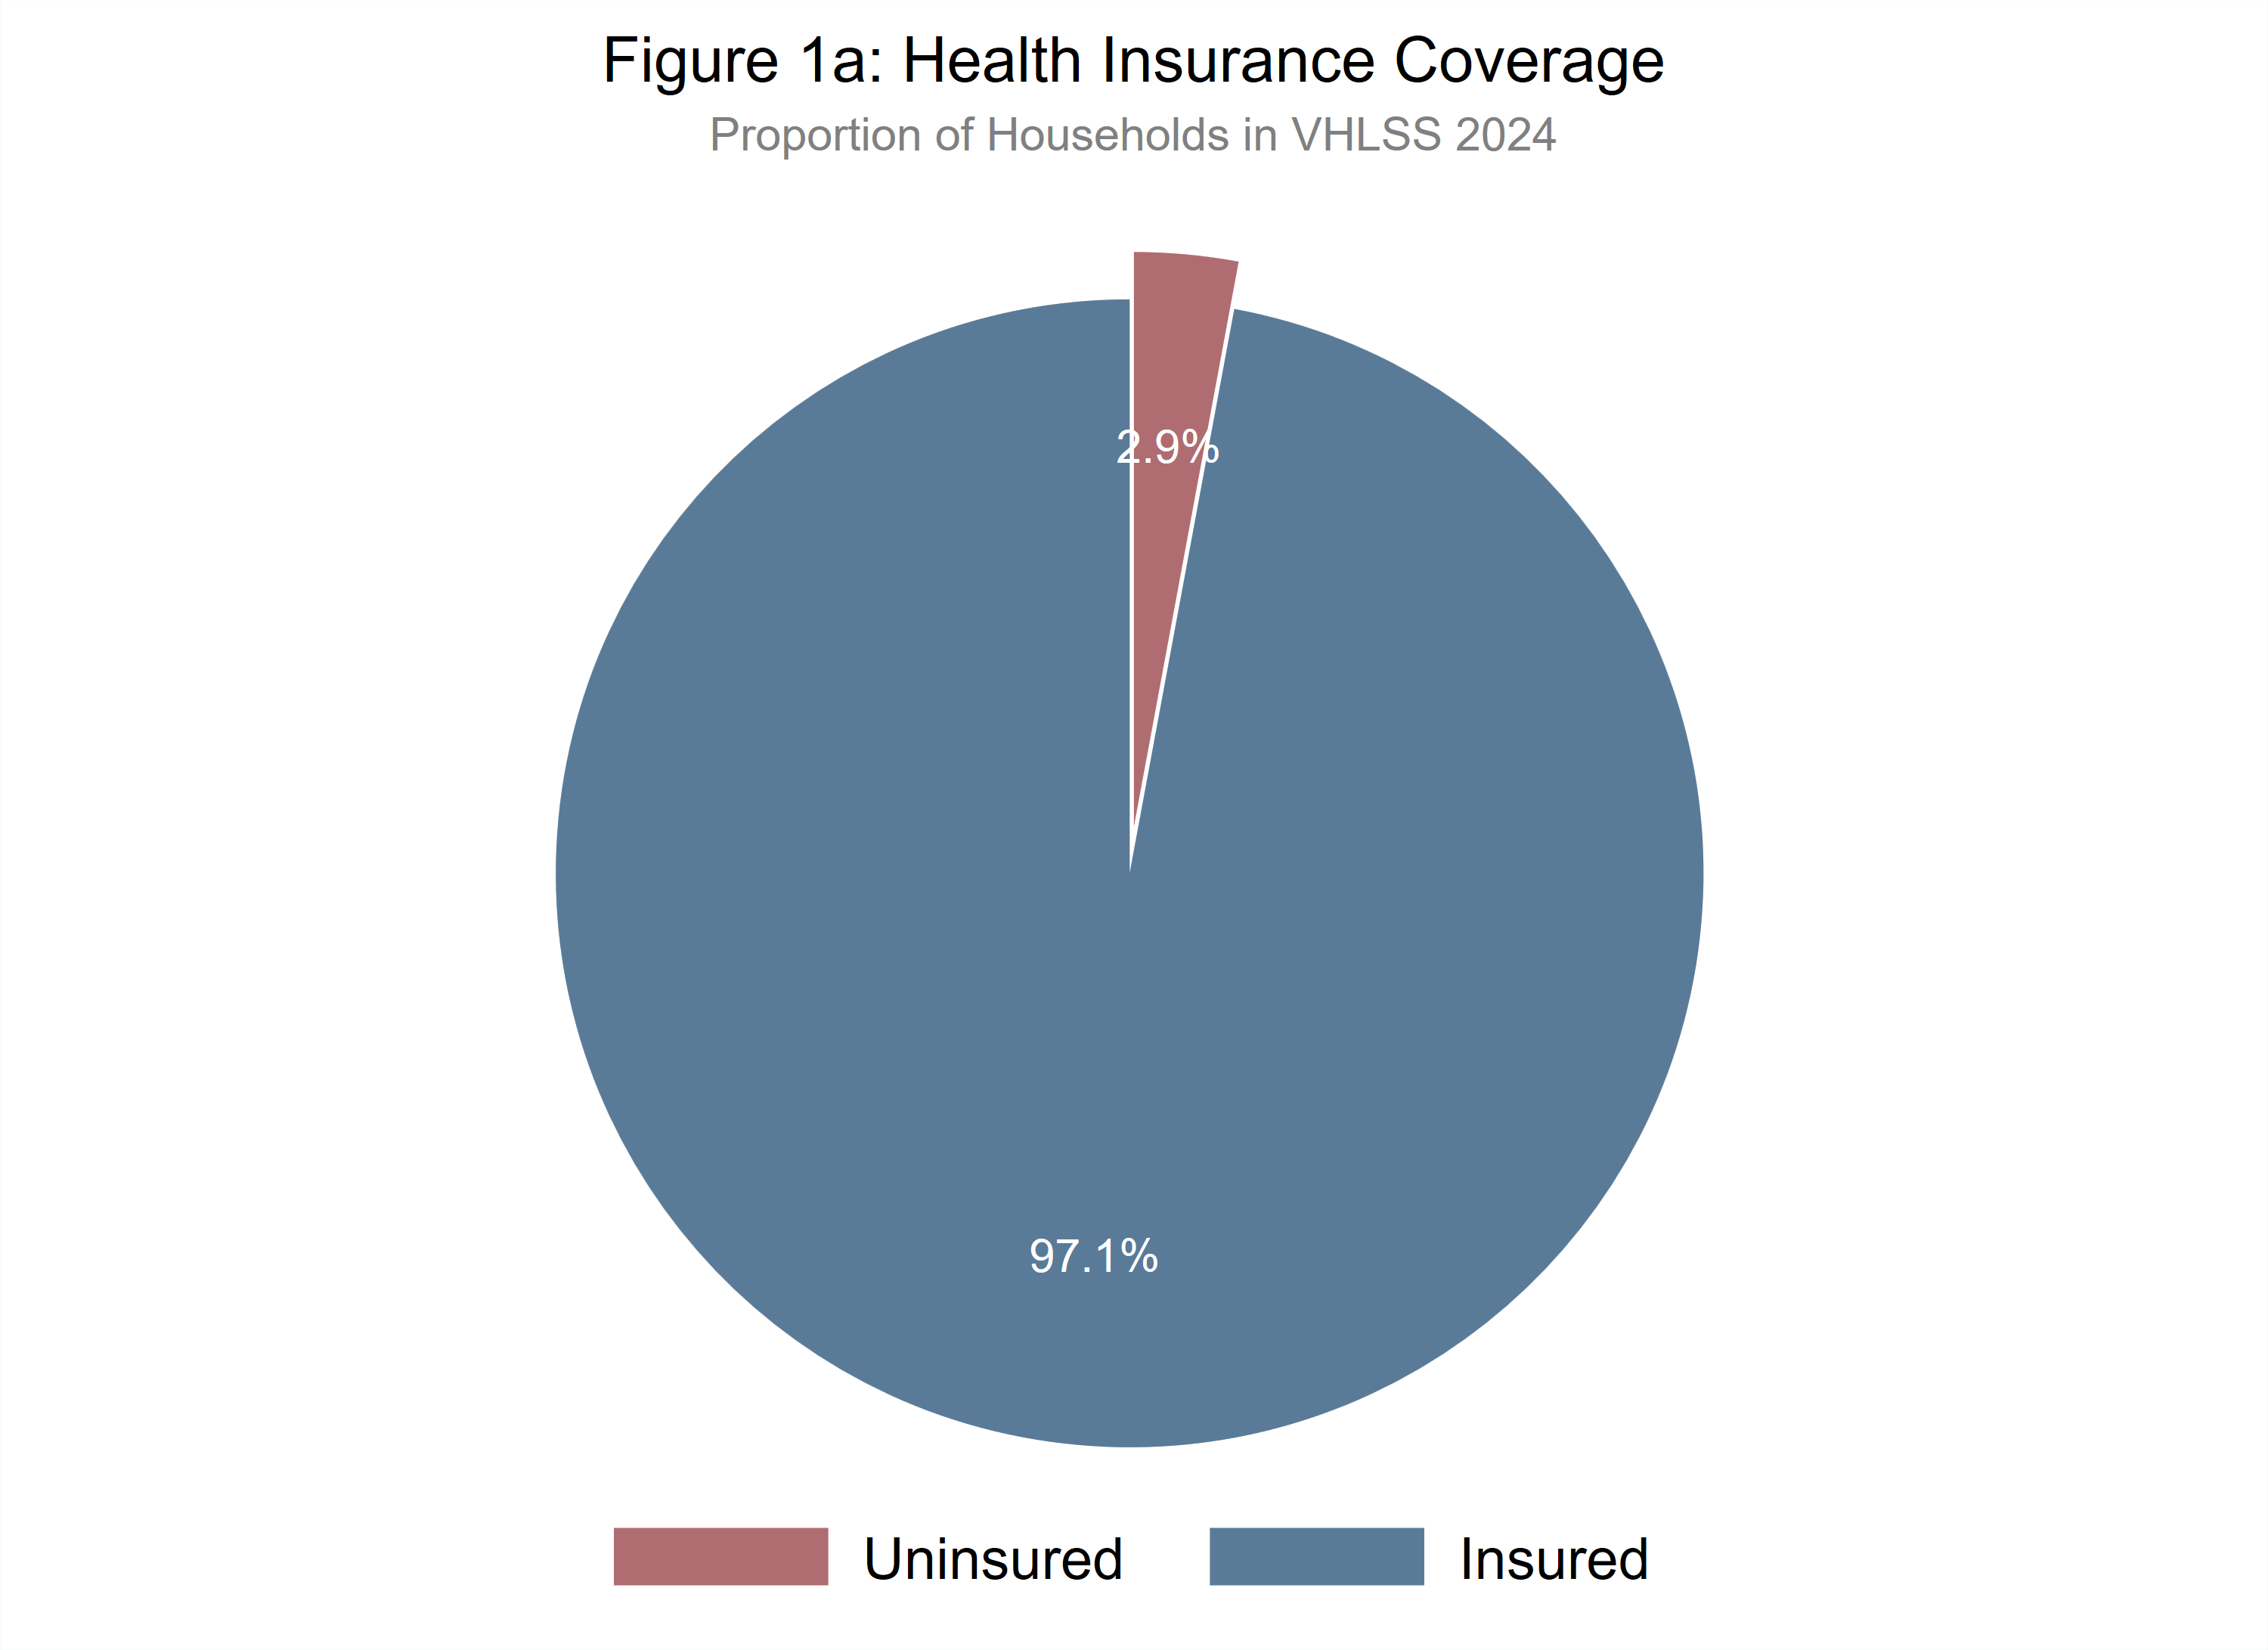
\includegraphics[width=0.75\textwidth]{Figure1a_Pie_BHYT.png}
	\caption{Tỷ lệ bao phủ Bảo hiểm Y tế của hộ gia đình (VHLSS 2024)}
	\label{fig:pie_bhyt}
\end{figure}

Về gánh nặng tài chính, trung bình mỗi hộ gia đình chi trả 5,578 triệu VNĐ/năm cho y tế tiền túi (OOP). Khi bóc tách cấu trúc này, chi phí khám chữa bệnh nội trú ($OOP_{in}$) và ngoại trú ($OOP_{out}$) trực tiếp tại cơ sở y tế lần lượt chiếm 1,495 triệu VNĐ và 1,341 triệu VNĐ. Đáng chú ý, , độ lệch chuẩn của chi phí nội trú ($10,278$) và giá trị tối đa cực đại ($600$ triệu VNĐ) cho thấy rủi ro tài chính thảm họa tập trung chủ yếu ở nhóm điều trị nội trú. Ngoài ra, có 37,5\% hộ gia đình có hành vi khám chữa bệnh vượt tuyến, đây là biến số quan trọng dự kiến sẽ làm thay đổi đáng kể hiệu ứng bảo vệ của BHYT trong các mô hình hồi quy tiếp theo. Điều này cho thấy rằng phần chênh lệch đáng kể còn lại phản ánh thói quen tự mua thuốc điều trị và vật tư y tế ngoài danh mục chi trả của người dân, một khu vực mà hệ thống BHYT hiện tại vẫn chưa bao phủ toàn diện, tiềm ẩn rủi ro tài chính đối với các hộ gia đình khi đối mặt với các bệnh mãn tính hoặc điều trị dài ngày. Đáng chú ý, có tới 37,5\% hộ gia đình ghi nhận hành vi tự ý khám chữa bệnh vượt tuyến, một yếu tố tiềm ẩn nguy cơ làm gia tăng hình phạt đồng chi trả. Để bóc tách sự phân hóa này (Hình \ref{fig:stacked_oop}) minh họa cấu trúc chi phí OOP theo đặc điểm không gian và hành vi khám chữa bệnh. 


% --- ĐỒ THỊ STACKED BAR ---
\begin{figure}[htbp]
	\centering
	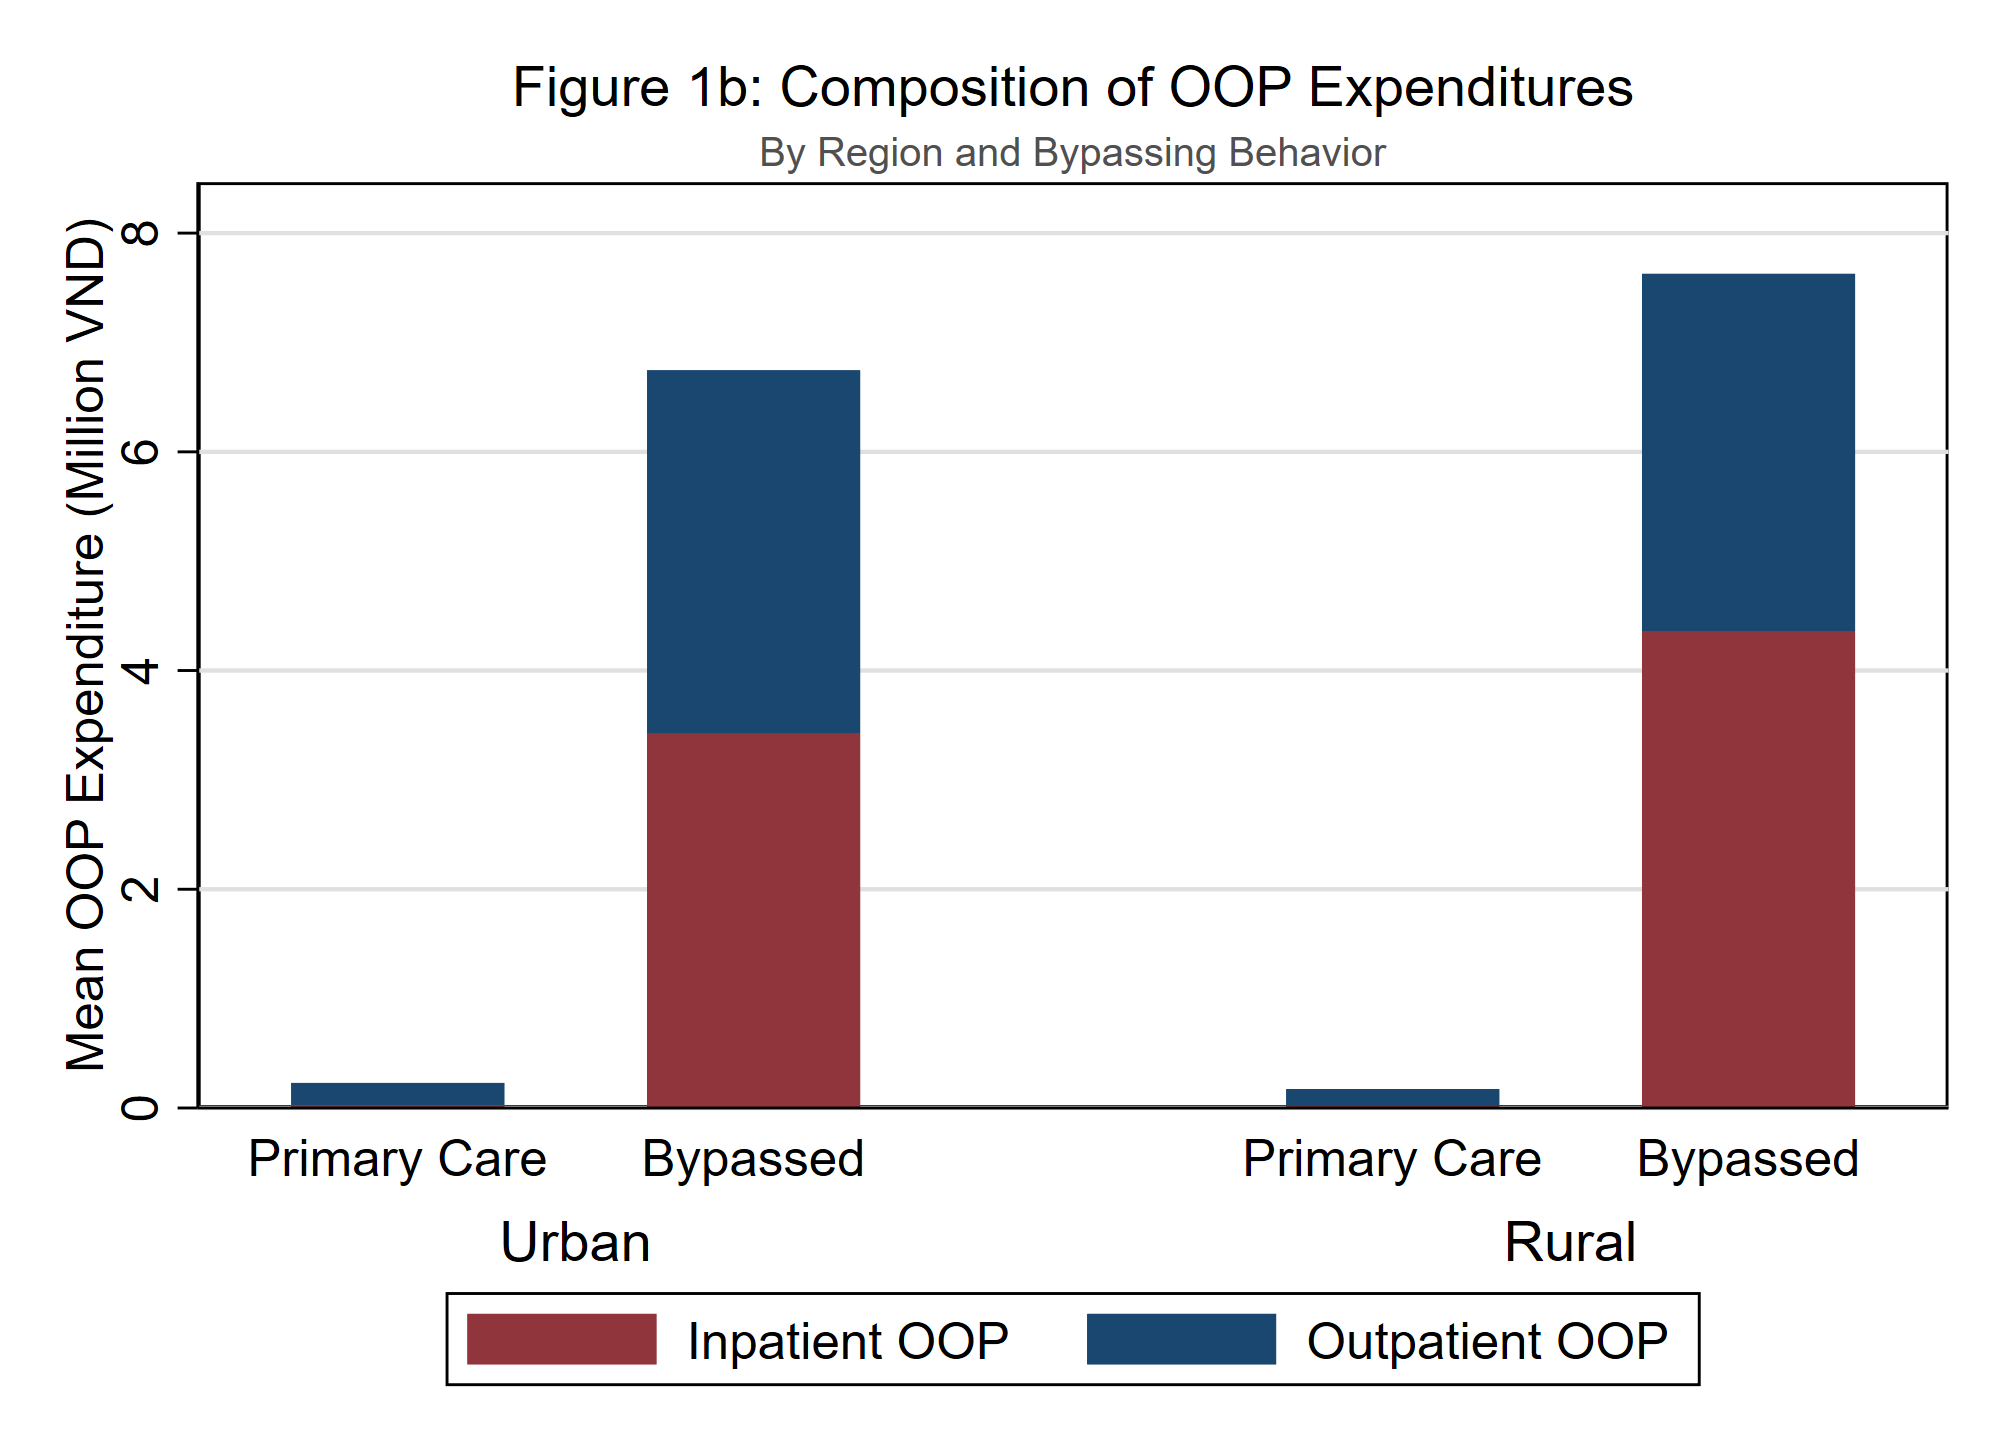
\includegraphics[width=0.85\textwidth]{figures/Figure1b_StackedBar_OOP.png}
	\caption{Cấu trúc chi phí y tế tiền túi (Nội trú vs. Ngoại trú) phân theo Khu vực và Hành vi vượt tuyến}
	\label{fig:stacked_oop}
\end{figure}


Dữ liệu thống kê mô tả trên bộc lộ một thực tế bất đối xứng sắc nét: Tại khu vực nông thôn, nhóm vượt tuyến phải gánh chịu sự bùng nổ của chi phí OOP nội trú. Hiện tượng này hàm ý rằng người dân vùng nông thôn thường chỉ chấp nhận chi phí tài chính rất cao để vượt tuyến y tế trên khi đối mặt với các cú sốc sức khỏe nghiêm trọng. Trong khi các nhu cầu ngoại trú được xử lý tại tuyến cơ sở. Ngược lại, tại khu vực thành thị, hành vi vượt tuyến thúc đẩy mạnh mẽ cả chi phí nội trú và ngoại trú, phản ánh khả năng tiếp cận y tế chuyên sâu dễ dàng hơn và có thể là dấu hiệu của rủi ro đạo đức trong sử dụng dịch vụ ngoại trú.

% --- ĐỒ THỊ BOXPLOT ---
\begin{figure}[htbp]
	\centering
	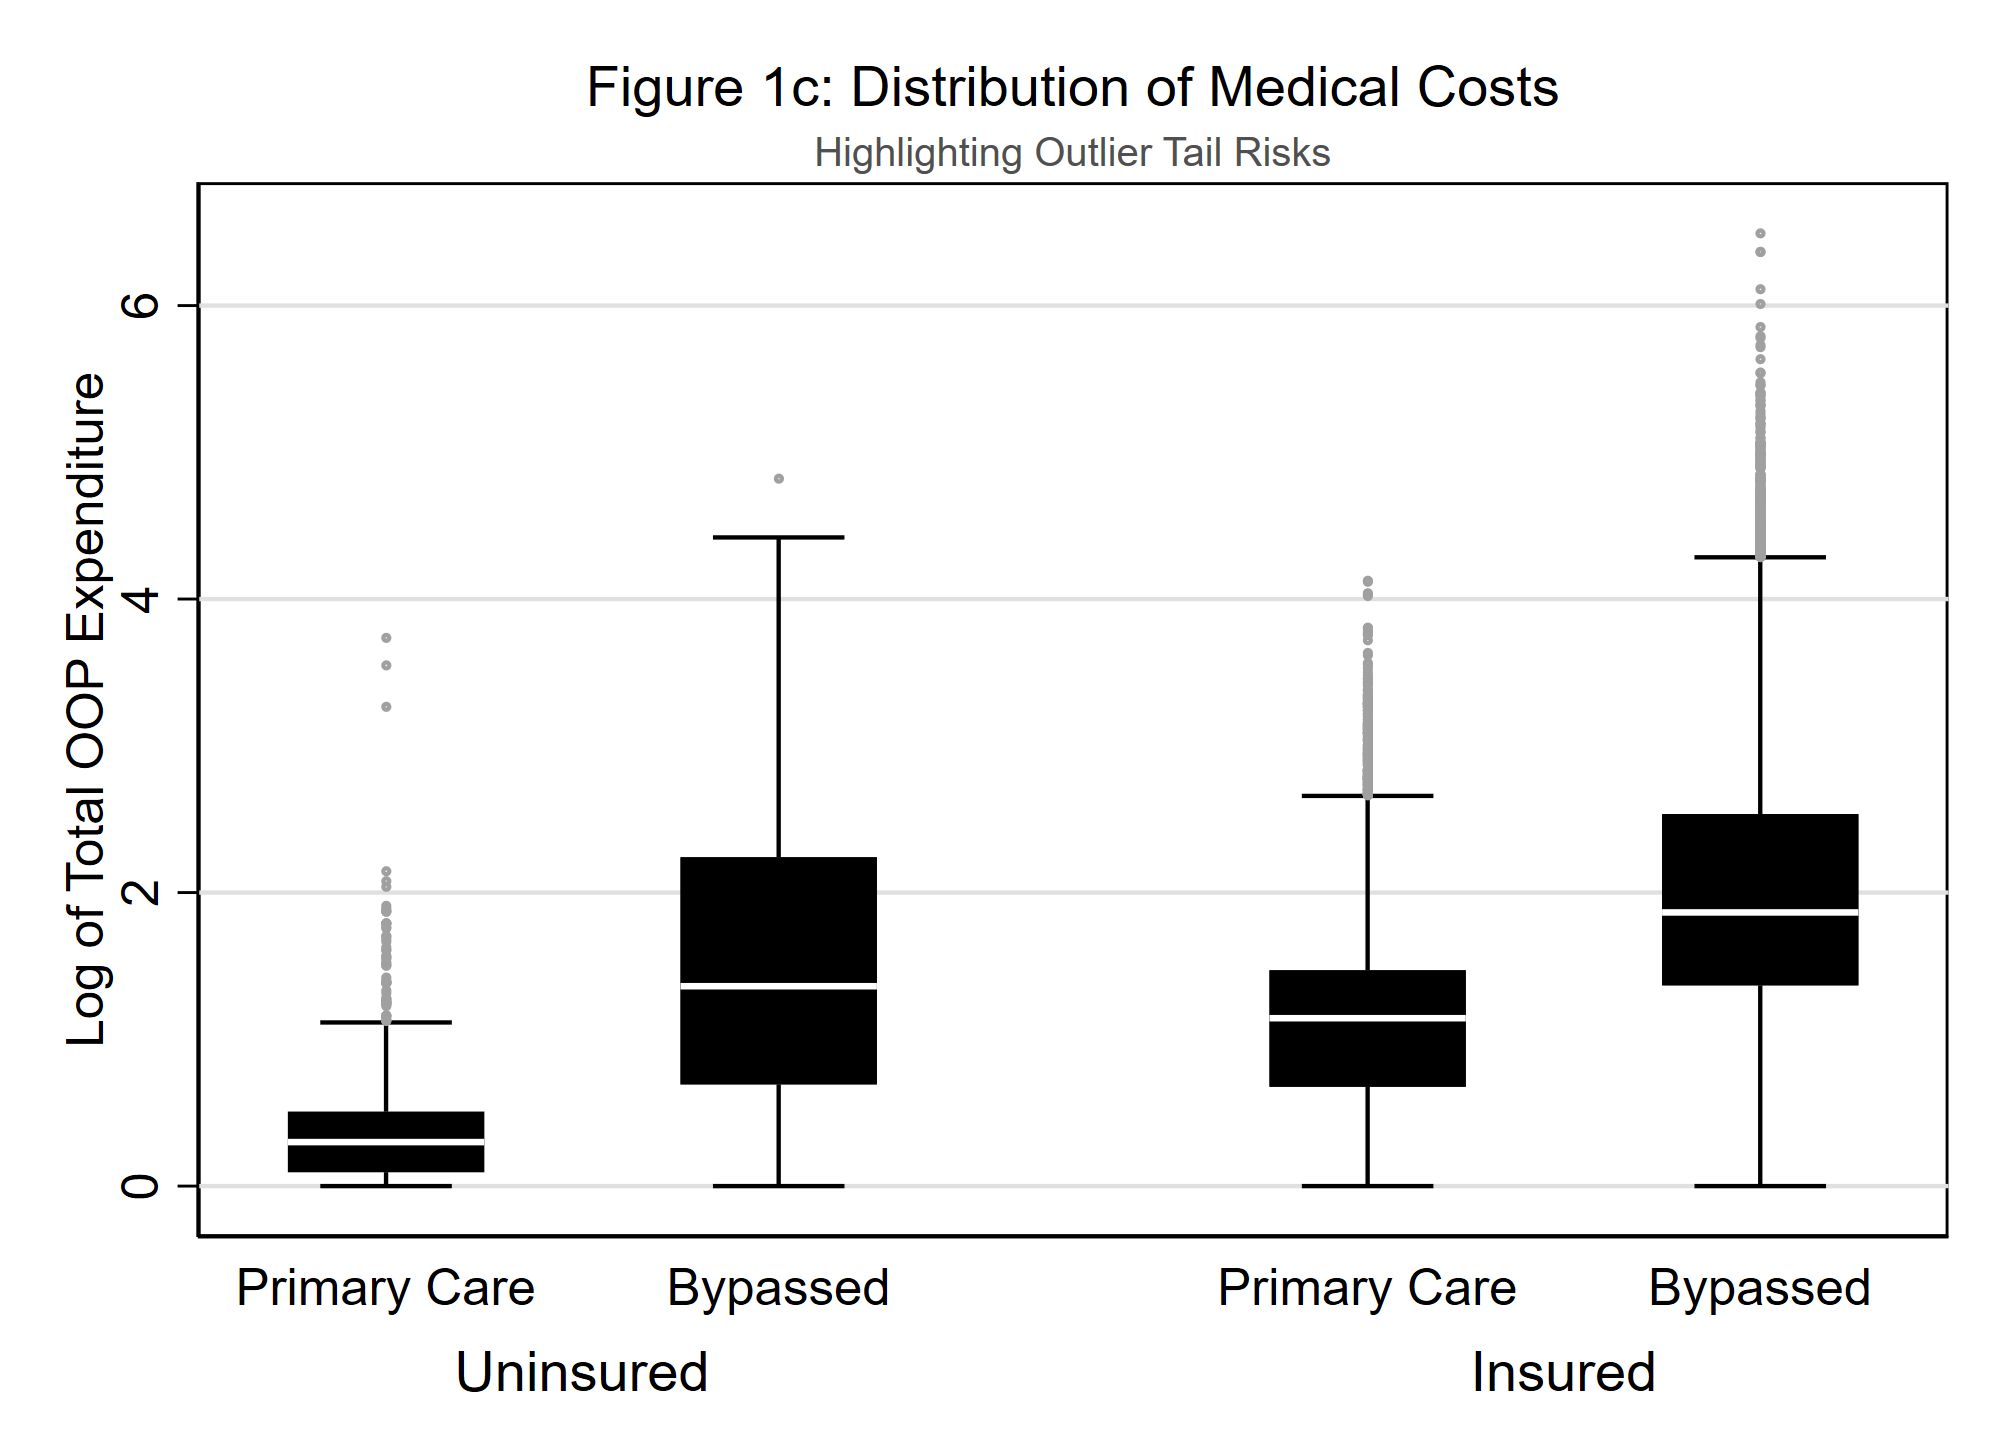
\includegraphics[width=0.85\textwidth]{figures/Figure1c_Boxplot_Bypass.png}
	\caption{Phân phối Log(OOP) nhấn mạnh rủi ro thảm họa y tế ở phần đuôi (Tail Risks)}
	\label{fig:boxplot_oop}
\end{figure}

Đặc điểm nổi bật nhất của chi phí OOP là sự phân phối lệch phải cực đoan. Với độ lệch chuẩn tổng thể lên tới 13,040 triệu VND, mức chi tối đa ghi nhận hàng trăm triệu đồng. Hình \ref{fig:boxplot_oop} sử dụng biểu đồ hộp (Boxplot) trên thang đo logarit để làm nổi bật rủi ro này. Có thể thấy rõ sự tồn tại của một tập hợp các điểm dị biệt phân bố dày đặc ở phần đuôi trên của mọi nhóm, đại diện cho các hộ gia đình rơi vào thảm họa y tế. Nhóm khám vượt tuyến không chỉ có mức chi phí trung vị cao hơn hẳn mà còn mở rộng phổ rủi ro ở phần đuôi so với nhóm tuân thủ khám tại tuyến cơ sở.

% --- ĐỒ THỊ KERNEL DENSITY ---
\begin{figure}[htbp]
	\centering
	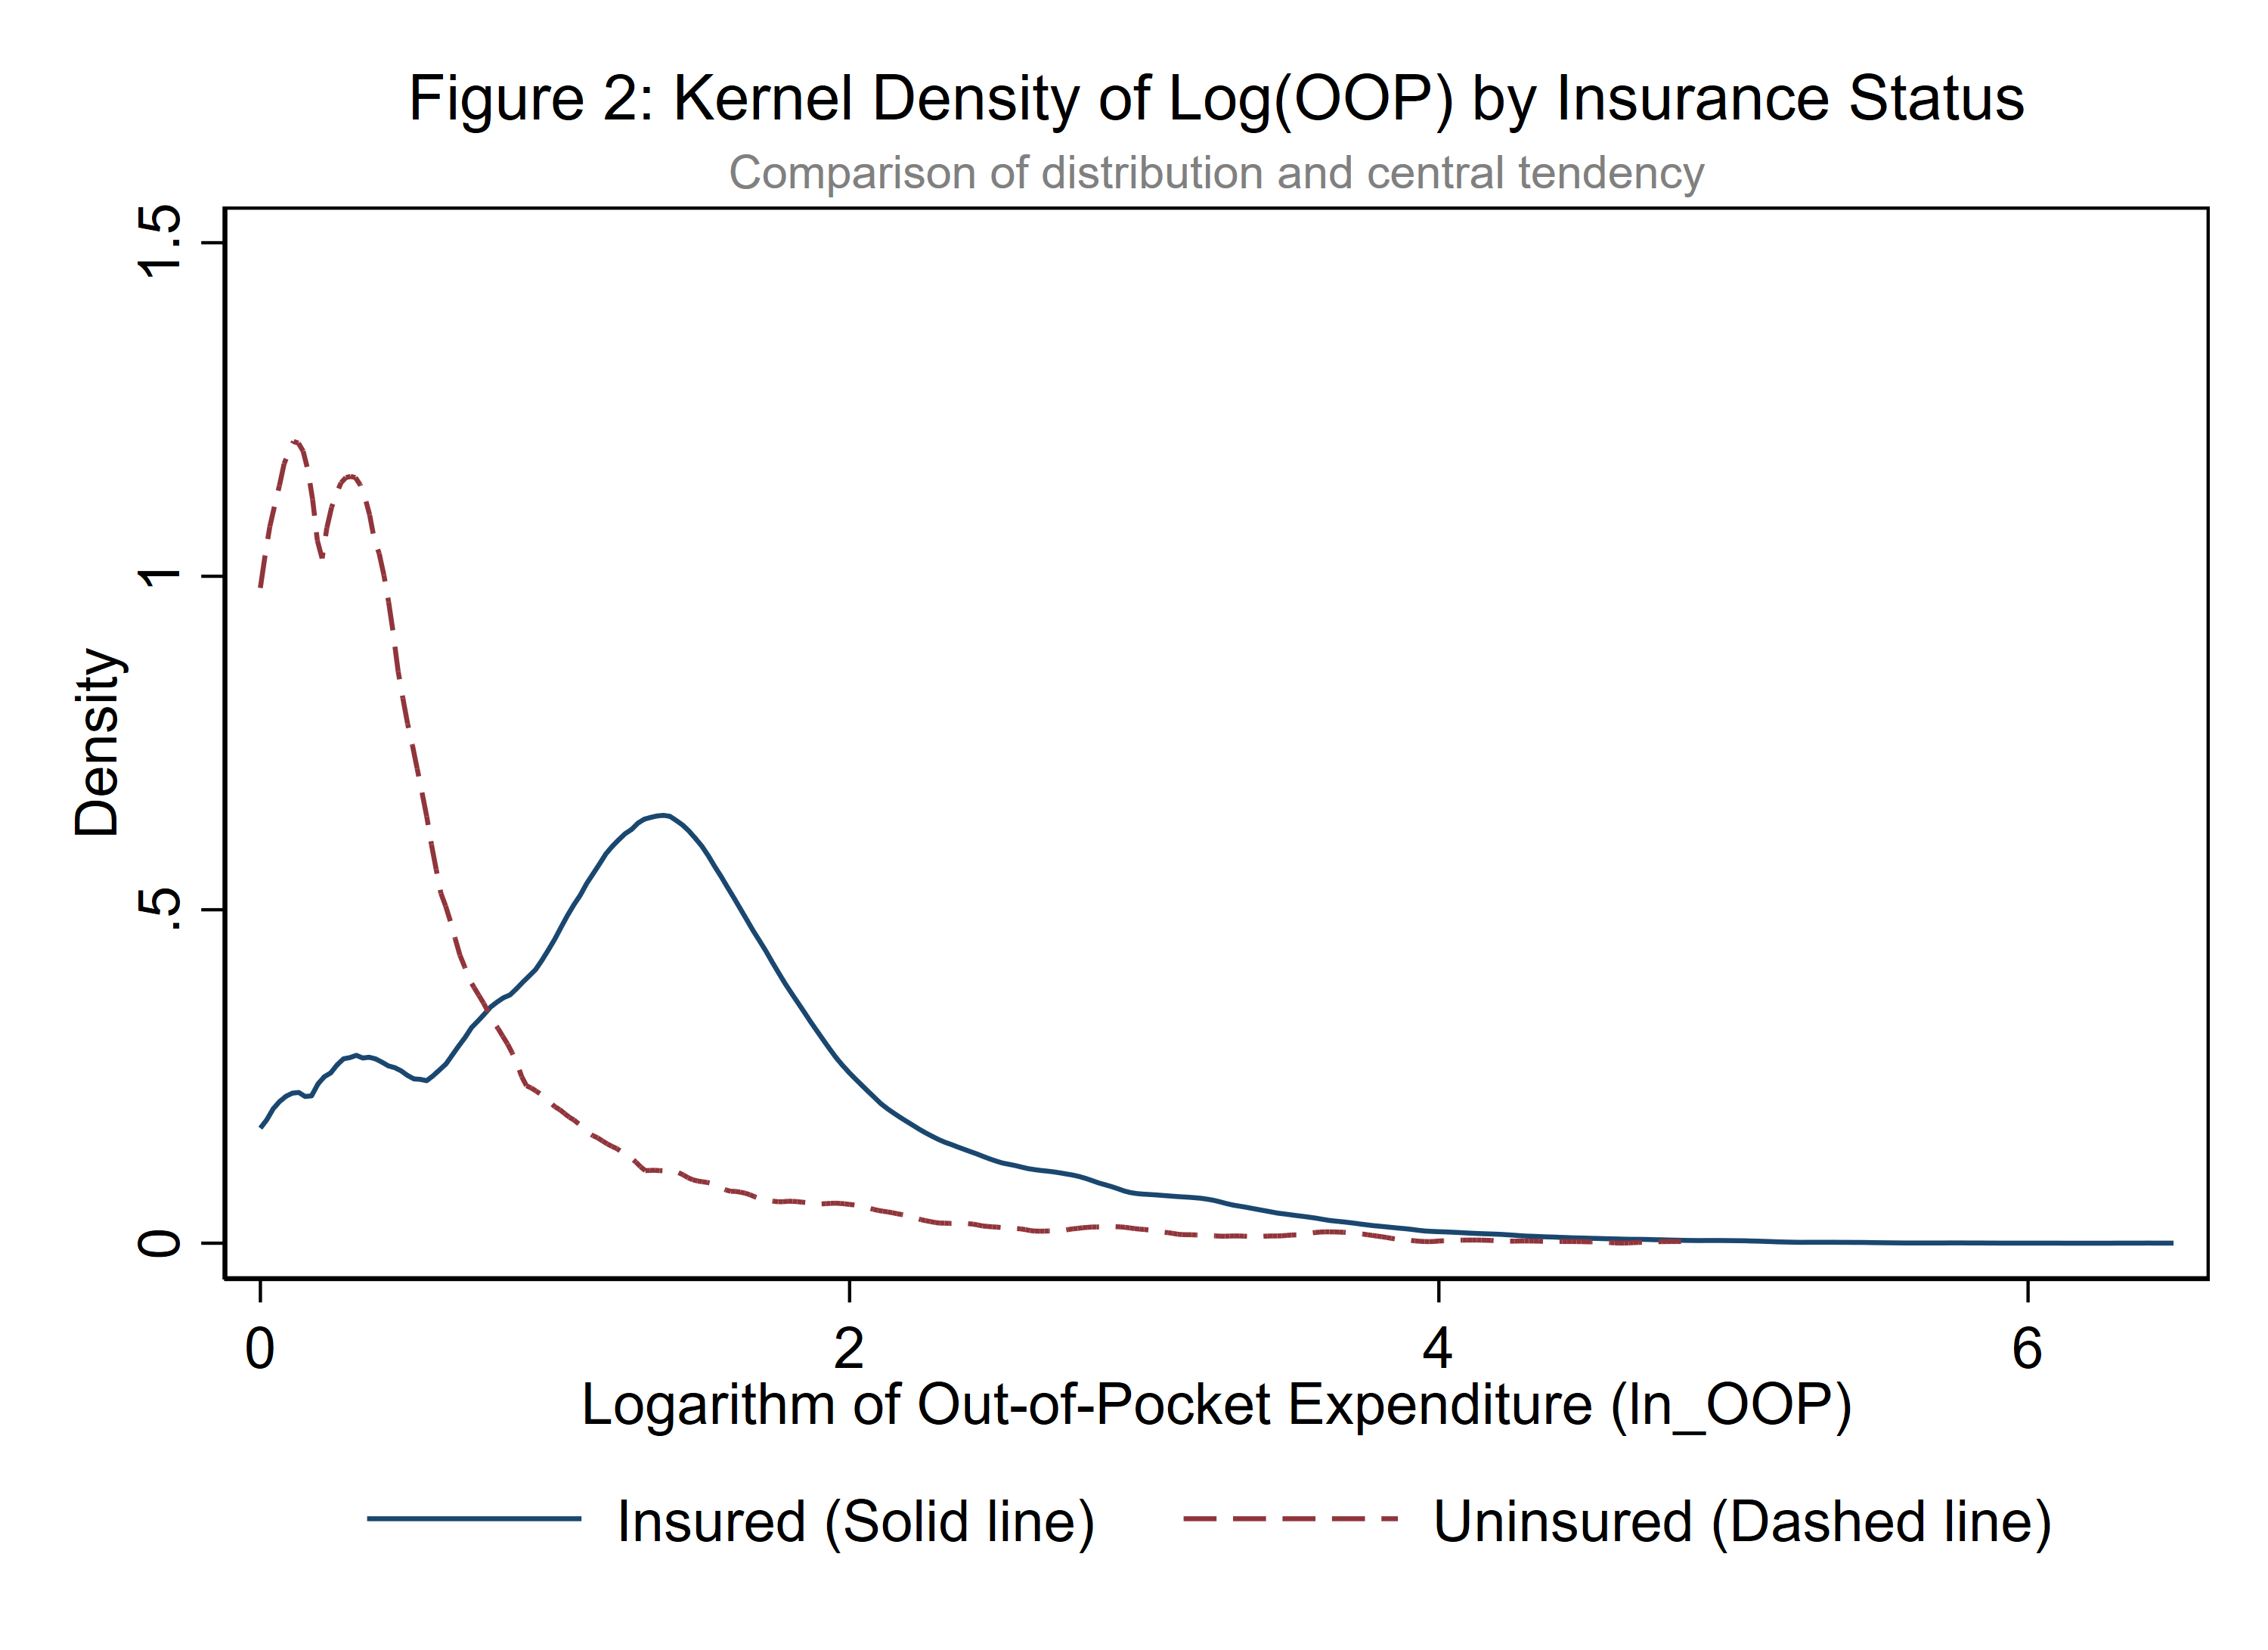
\includegraphics[width=0.8\textwidth]{figures/Figure2_Kernel_Density.png}
	\caption{Phân phối mật độ (Kernel Density) của Log chi tiêu y tế tiền túi theo trạng thái BHYT}
	\label{fig:kernel_density}
\end{figure}

Việc sử dụng dạng hàm logarit ($\ln\_OOP$) là bước chuyển hóa cần thiết để xử lý đặc tính lệch phải cực đoan và kéo phân phối về dạng tiệm cận chuẩn (Hình \ref{fig:kernel_density}). Nhìn trực quan, đường mật độ của nhóm có BHYT (nét liền) dịch chuyển rõ rệt sang phải ở phần thân phân phối so với nhóm không có BHYT (nét đứt). Mức chi phí OOP trung bình của nhóm có BHYT (5,705 triệu VND) cũng cao hơn nhóm không có BHYT (1,501 triệu VND). 

Sự dịch chuyển này củng cố giả thuyết về hiệu ứng kép của BHYT: Một mặt, nó kích thích giải phóng nhu cầu y tế (đặc biệt khi kết hợp với hành vi vượt tuyến), đẩy tổng chi phí trung bình lên cao; mặt khác, hình dáng phân phối (Boxplot và Kernel) cho thấy tiềm năng nén lại các cú sốc cực đoan. Tuy nhiên, để định lượng chính xác hiệu ứng bảo vệ này, đồng thời giải quyết triệt để vấn đề nội sinh do tự lựa chọn tham gia BHYT, việc áp dụng mô hình biến công cụ (IV-2SLS) là bước phân tích bắt buộc trong phần tiếp theo.

Tóm lại, những phát hiện từ thống kê mô tả và phân tích trực quan đã phác họa rõ nét gánh nặng chi phí y tế tiền túi cùng rủi ro thảm họa ở đuôi phân phối, đồng thời hé lộ những tín hiệu ban đầu về tác động phức tạp của BHYT và hành vi vượt tuyến, từ đó, tạo tiền đề để tiến tới phân tích định lượng các mối quan hệ nhân quả này thông qua các mô hình kinh tế lượng ở phần tiếp theo.

\newpage
\subsection{Hiệu ứng kép của BHYT qua lăng kính phân rã chi phí (IV-2SLS)}

Kết quả từ mô hình IV-2SLS (Bảng \ref{tab:decomposed_oop}) chứng minh một cách mạnh mẽ sự tồn tại của "Hiệu ứng kép" (Dual Effect) có tính chất phi tuyến trong cơ chế vận hành của BHYT.

\begin{table}[htbp]
	\centering
	\def\sym#1{\ifmmode^{#1}\else\(^{#1}\)\fi}
	\caption{Tác động của BHYT lên cấu trúc chi phí OOP phân rã (Mô hình IV-2SLS)}
	\label{tab:decomposed_oop}
	\begin{tabular}{lccc}
		\toprule
		&\textbf{(1)}&\textbf{(2)}&\textbf{(3)}\\
		\textbf{Biến độc lập}&\textbf{Log(Tổng OOP)}&\textbf{Log(OOP Nội trú)}&\textbf{Log(OOP Ngoại trú)}\\
		\midrule
		BHYT (Cơ sở) & 1.256\sym{***} & -0.219 & 0.292\sym{*} \\
		& (0.177) & (0.155) & (0.157) \\
		\addlinespace
		BHYT $\times$ Nông thôn & -0.967\sym{***} & -0.115 & 0.035 \\
		& (0.286) & (0.178) & (0.137) \\
		\addlinespace
		BHYT $\times$ Vượt tuyến & 2.413 & 2.806 & 0.405 \\
		& (1.833) & (2.172) & (1.513) \\
		\addlinespace
		BHYT $\times$ Nông thôn $\times$ Vượt tuyến & -3.533 & -1.345 & -2.971\sym{*} \\
		& (2.151) & (2.431) & (1.707) \\
		\addlinespace
		Nông thôn (Base) & 0.850\sym{***} & 0.083 & -0.026 \\
		& (0.262) & (0.155) & (0.133) \\
		\addlinespace
		Vượt tuyến (Base) & -1.648 & -2.244 & 0.443 \\
		& (1.795) & (2.092) & (1.493) \\
		\midrule
		Biến kiểm soát ($X$) & Có & Có & Có \\
		Fixed Effects (Tỉnh) & Có & Có & Có \\
		\midrule
		Số quan sát ($N$) & 46.995 & 46.995 & 46.995 \\
		\bottomrule
		\multicolumn{4}{p{13cm}}{\footnotesize \textit{Ghi chú:} Sai số chuẩn vững (Robust standard errors) được cụm theo cấp tỉnh đặt trong ngoặc đơn. \newline \sym{*} \(p<0.10\), \sym{**} \(p<0.05\), \sym{***} \(p<0.01\)}
	\end{tabular}
\end{table}

% --- ĐỒ THỊ FOREST PLOT (HIỆU ỨNG KÉP) ---
\begin{figure}[htbp]
	\centering
	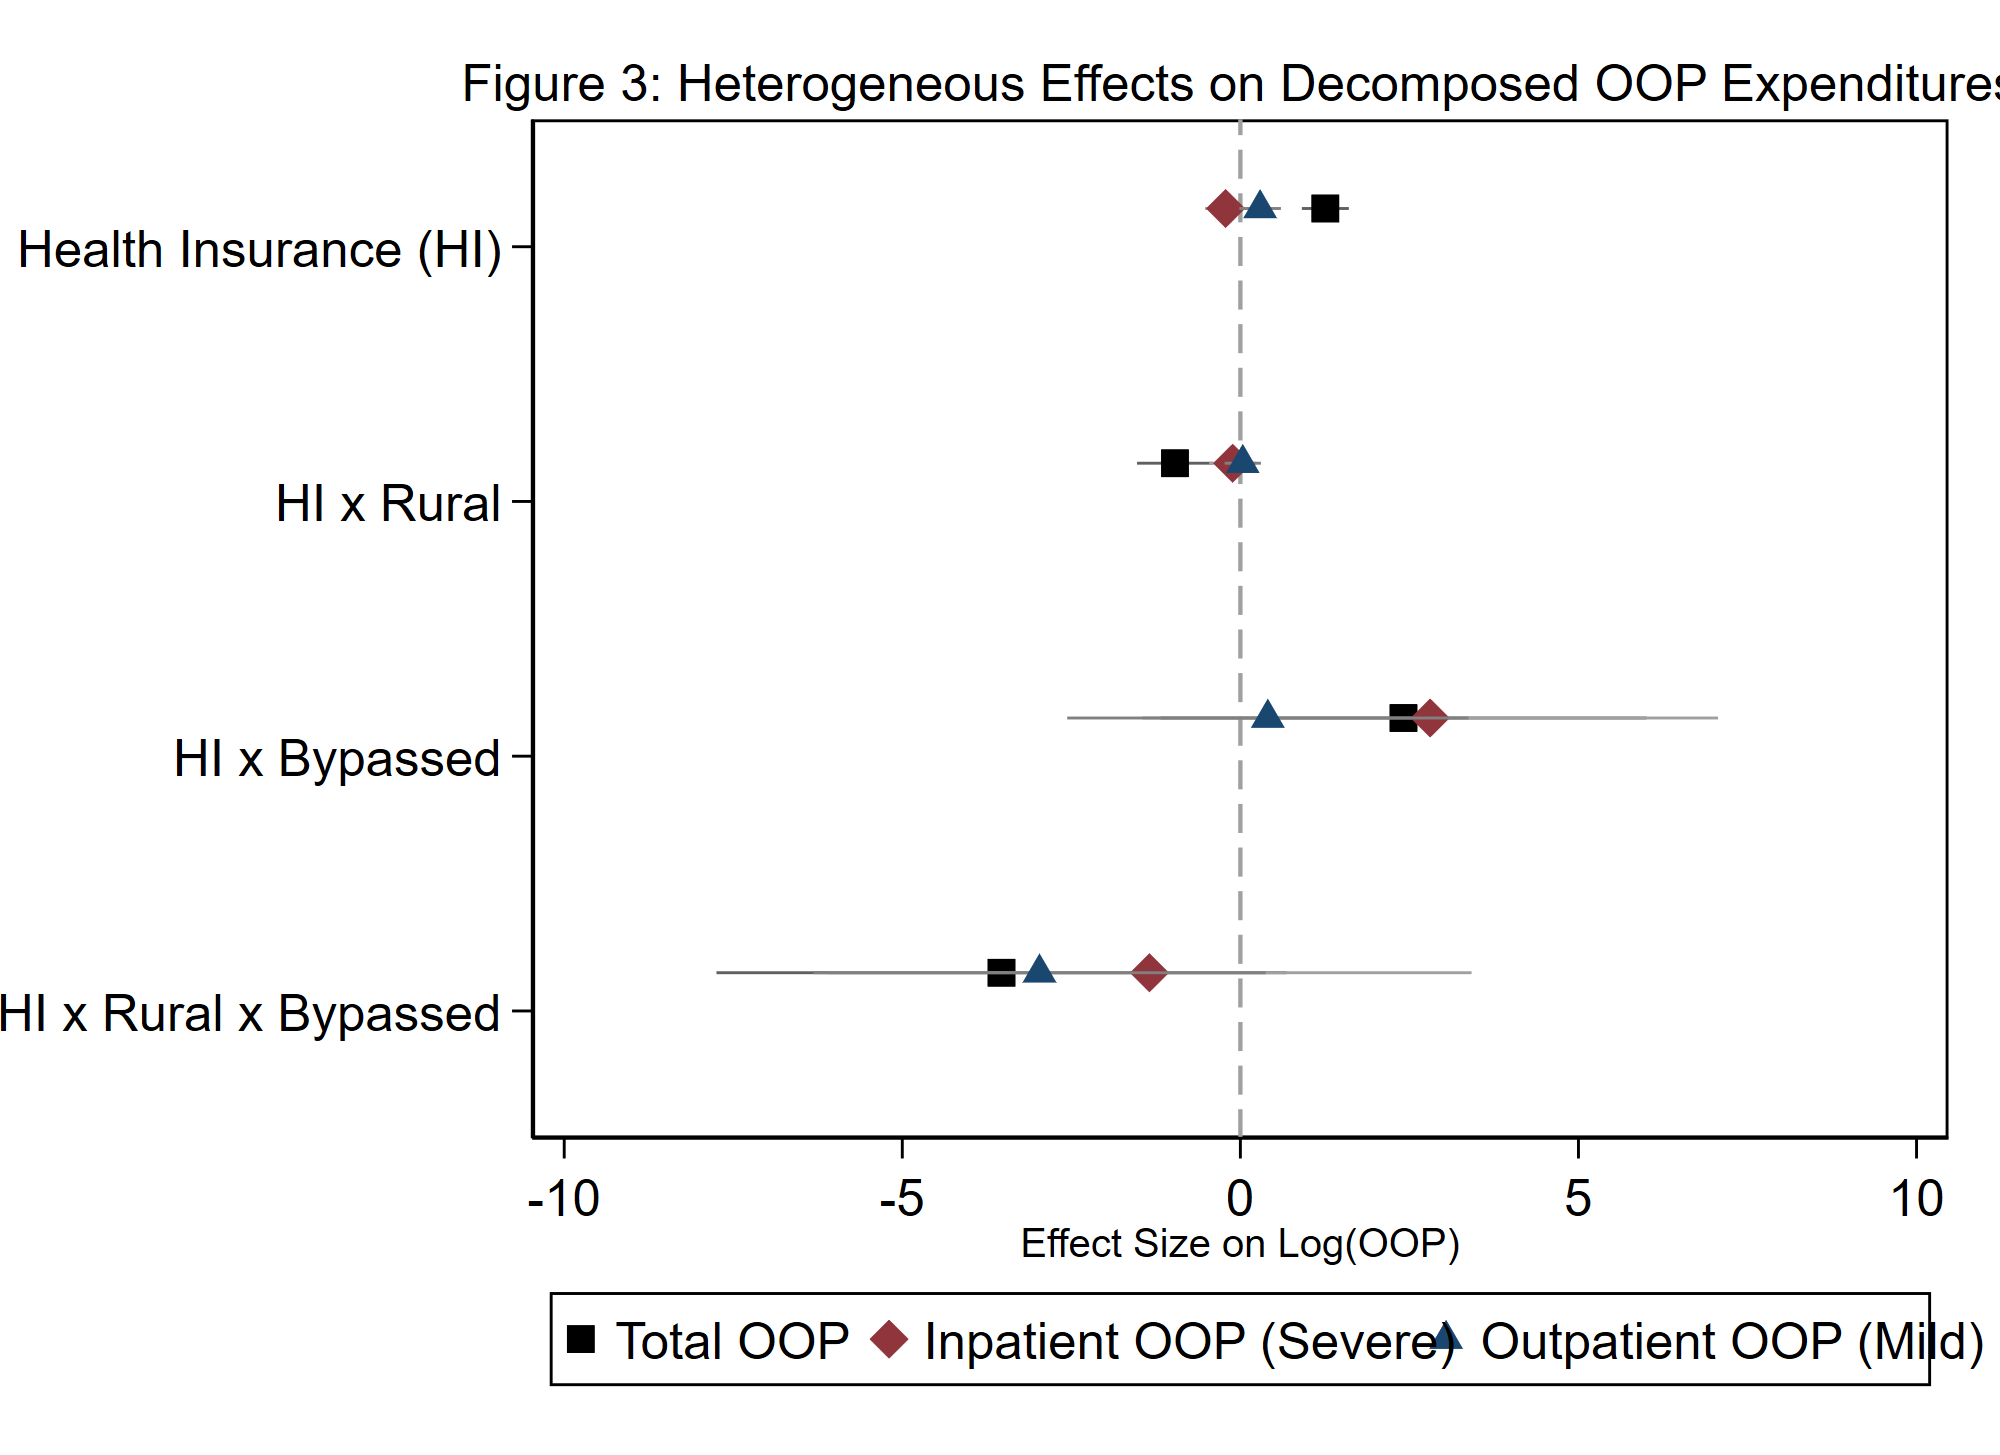
\includegraphics[width=0.9\textwidth]{figures/Figure3_Combined_ForestPlot.png}
	\caption{Hiệu ứng phân hóa của BHYT lên cấu trúc chi phí OOP (Combined Forest Plot)}
	\label{fig:forest_plot}
\end{figure}

Sự đối lập trong cơ chế tác động của BHYT được biểu diễn trực quan thông qua Forest Plot (Hình \ref{fig:forest_plot}), phơi bày hai mảng "sáng - tối" của chính sách:

\begin{itemize}
	\item \textbf{Kích thích tiếp cận ở Ngoại trú (Hiệu ứng mở rộng):} Ở Cột (3), hệ số BHYT cơ sở mang dấu dương ($+0.292, p < 0.10$). Điều này xác nhận rằng với các dịch vụ nhẹ, việc sở hữu thẻ BHYT đã gỡ bỏ rào cản tài chính ban đầu, khai thông lượng nhu cầu y tế vốn bị kìm nén trước đây. Sự gia tăng tần suất sử dụng dịch vụ kéo theo sự phình to của các khoản đồng chi trả và chi phí tự mua thuốc bên ngoài, làm tăng mức OOP ngoại trú nói chung.
	\item \textbf{Lưới an sinh tại Nông thôn và Tác động răn đe khi Vượt tuyến:} Trái ngược với hiệu ứng tăng chi phí ở nhóm cơ sở, BHYT thể hiện sức mạnh bảo vệ tài chính (financial protection) rõ rệt đối với các nhóm yếu thế. Tại Cột (1), tương tác 2 chiều ($BHYT \times N\hat{o}ng\ th\hat{o}n$) tạo ra lực cản giảm Tổng OOP rất mạnh ($-0.967, p < 0.01$). Đặc biệt hơn, tại Cột (3), biến tương tác 3 chiều ($BHYT \times N\hat{o}ng\ th\hat{o}n \times V\mathopen{ư}\mathclose{ợ}t\ tuy\acute{ế}n$) ghi nhận mức giảm kỷ lục ($-2.971, p < 0.10$). Điều này mang hàm ý chính sách sâu sắc: Các cơ chế hình phạt tài chính của BHYT đối với hành vi vượt tuyến đang hoạt động cực kỳ hiệu quả ở nhóm bệnh nhân nông thôn trong các ca ngoại trú, giúp định tuyến bệnh nhân và ngăn chặn tình trạng đổ xô lên tuyến trên không cần thiết.
	\item \textbf{Khoảng trống trong bảo vệ Nội trú:} Đáng chú ý, toàn bộ các hệ số tại Cột (2) (OOP Nội trú) đều không đạt mức ý nghĩa thống kê. Thay vì vội vã kết luận BHYT không có tác dụng, sự thiếu vắng ý nghĩa thống kê này phản ánh một thực tế lâm sàng: chi phí điều trị nội trú có độ phân tán (variance) vô cùng cực đoan. Khi một bệnh nhân rơi vào cảnh thảm họa y tế cần nằm viện dài ngày, các giới hạn trần thanh toán và danh mục thuốc ngoài BHYT khiến thẻ bảo hiểm chưa thể hiện được sự khác biệt tuyến tính trên mức trung bình mẫu. Điều này đòi hỏi các phân tích chuyên sâu hơn ở phần đuôi của phân phối chi phí (được giải quyết thông qua mô hình SQREG ở phần tiếp theo).
\end{itemize}

\subsection{Tác động dọc theo phân phối thảm họa (SQREG)}

Để đánh giá sự thay đổi trong cơ chế bảo vệ của BHYT khi đối mặt với các cú sốc y tế lớn, nghiên cứu sử dụng mô hình Hồi quy phân vị đồng thời (SQREG). Bảng \ref{tab:sqreg_summary} tóm tắt các hệ số trọng tâm được trích xuất từ mô hình đầy đủ (Phụ lục B).

\begin{table}[htbp]
	\centering
	\def\sym#1{\ifmmode^{#1}\else\(^{#1}\)\fi}
	\caption{Tóm tắt tác động của BHYT và hành vi Vượt tuyến theo phân vị chi phí}
	\label{tab:sqreg_summary}
	\begin{tabular}{lcccc}
		\toprule
		&\textbf{(1)}&\textbf{(2)}&\textbf{(3)}&\textbf{(4)}\\
		\textbf{Biến độc lập}&\textbf{Q25}&\textbf{Q50}&\textbf{Q75}&\textbf{Q90}\\
		\midrule
		Vượt tuyến & 0.558\sym{***} & 0.916\sym{***} & 1.654\sym{***} & 2.039\sym{***} \\
		& (0.081) & (0.088) & (0.121) & (0.228) \\
		\addlinespace
		BHYT $\times$ Vượt tuyến & -0.045 & -0.290\sym{***} & -0.643\sym{***} & -0.605\sym{***} \\
		& (0.083) & (0.090) & (0.125) & (0.228) \\
		\midrule
		Các biến kiểm soát & Có & Có & Có & Có \\
		\midrule
		Pseudo $R^2$ & 0.202 & 0.209 & 0.260 & 0.314 \\
		Số quan sát ($N$) & \multicolumn{4}{c}{46.995} \\
		\bottomrule
		\multicolumn{5}{p{13cm}}{\footnotesize \textit{Ghi chú:} Bảng chỉ hiển thị các hệ số trọng tâm. Kết quả chi tiết xem tại Phụ lục B. Sai số chuẩn bootstrap (100 lần lặp) trong ngoặc đơn. \sym{***} \(p<0.01\)}
	\end{tabular}
\end{table}


Kết quả SQREG xác nhận sự leo thang tuyến tính của "hình phạt vượt tuyến" dọc theo phân phối chi phí. Cụ thể, hệ số của hành vi vượt tuyến tăng phi mã từ $0.558$ ở nhóm chi tiêu thấp ($Q25$) lên đến mức thảm họa $2.039$ ở đỉnh rủi ro ($Q90$). 

Đáng chú ý, chính tại phân vị cực đoan $Q90$ này, thẻ BHYT mới phát huy uy lực bảo vệ lớn nhất. Hệ số tương tác (BHYT $\times$ Vượt tuyến) chuyển từ trạng thái không có ý nghĩa thống kê ở $Q25$ sang mức cản phá mạnh mẽ $-0.605$ ($p < 0.01$) tại $Q90$. Điều này minh chứng rằng: Dù BHYT không ngăn được hoàn toàn chi phí dội lên do tự ý vượt tuyến, nó đóng vai trò như một chiếc "phanh hãm" khẩn cấp, cứu bệnh nhân khỏi nguy cơ phá sản y tế khi hóa đơn điều trị chạm ngưỡng thảm họa.

\subsection{Kiểm tra độ vững mô hình}

\subsubsection{Đánh giá tương quan tuyến tính và rủi ro đa cộng tuyến}

Nghiên cứu sử dụng Ma trận tương quan Pearson có trọng số (Bảng \ref{tab:corr_matrix}) và Hệ số phóng đại phương sai (VIF) để kiểm tra các mối quan hệ tuyến tính, qua đó phát hiện và xử lý rủi ro đa cộng tuyến. 

Kết quả ma trận tương quan cho thấy các đặc điểm dữ liệu phù hợp với kỳ vọng lý thuyết. Biến phụ thuộc là chi tiêu y tế từ tiền túi (\texttt{ln\_OOP}) có tương quan dương với hành vi khám chữa bệnh vượt tuyến (0.509) và quy mô hộ gia đình (0.284). Đáng chú ý, các biến độc lập đóng vai trò kiểm soát (như \texttt{ln\_INC}, \texttt{AGE\_HEAD}, \texttt{SEX\_HEAD}, \texttt{HH\_SIZE}) thể hiện tính độc lập cao khi các hệ số tương quan chéo đều ở mức rất thấp (giá trị tuyệt đối $< 0.3$). Sự độc lập này cũng được khẳng định qua kết quả VIF, khi tất cả các hiệp biến nhân khẩu học và kinh tế đều có giá trị VIF rất thấp ($< 1.3$).

Bên cạnh đó, ma trận ghi nhận hệ số tương quan gần như hoàn hảo ở một số cặp biến đặc thù, nổi bật là giữa \texttt{RURAL} và \texttt{ins\_rural} (0.966), hay \texttt{hh\_vuot\_tuyen} và \texttt{ins\_vuot} (0.992). Kết quả kiểm định VIF tại các biến này tương ứng cũng ở mức cao. Tuy nhiên, về mặt phương pháp luận, đây là hiện tượng đa cộng tuyến cấu trúc (structural multicollinearity) mang tính tất yếu do toán học (được nhân lên từ các biến gốc để tạo biến tương tác), hoàn toàn không phản ánh lỗi thiết lập mô hình hay làm sai lệch hệ số ước lượng.

Nhìn chung, với mức VIF trung bình của toàn mô hình chỉ đạt $4.14$ (thấp hơn đáng kể so với ngưỡng cảnh báo thông thường là 10), nghiên cứu kết luận rằng cấu trúc dữ liệu hoàn toàn hợp lệ và không vi phạm giả định về đa cộng tuyến nghiêm trọng.

\subsubsection{Kiểm định khuyết tật của mô hình}

Để đảm bảo tính vững và độ tin cậy của các mô hình, nghiên cứu đã tiến hành kiểm tra hai khuyết tật phổ biến trong dữ liệu vi mô cắt ngang: Phương sai sai số thay đổi (heteroskedasticity) và Tương quan nội cụm (intra-cluster correlation).

Thứ nhất, đối với hiện tượng phương sai sai số thay đổi, do mô hình sử dụng phương pháp biến công cụ (IV-2SLS), nghiên cứu áp dụng kiểm định Pagan-Hall thay cho kiểm định Breusch-Pagan truyền thống để đảm bảo tính hợp lệ khi có sự xuất hiện của biến nội sinh. Kết quả cho thấy thống kê Pagan-Hall đạt mức 2982.26 với giá trị $p < 0.001$, qua đó bác bỏ mạnh mẽ giả thuyết không ($H_0$) về phương sai đồng nhất. Điều này xác nhận sự hiện diện của hiện tượng phương sai sai số thay đổi trong cấu trúc dữ liệu.

Thứ hai, do dữ liệu khảo sát được thu thập theo các địa bàn cấp tỉnh, các hộ gia đình trong cùng một tỉnh có xu hướng chia sẻ các đặc điểm chung không quan sát được về chính sách y tế và chất lượng cơ sở hạ tầng. Phân tích phương sai một chiều (One-way ANOVA) chỉ ra hệ số tương quan nội cụm (Intraclass Correlation Coefficient - ICC) đạt giá trị 0.0705. Nghĩa là, khoảng 7.06\% sự biến thiên của chi tiêu y tế từ tiền túi được giải thích bởi hiệu ứng riêng biệt cấp tỉnh. Thống kê F có ý nghĩa ở mức 1\% ($p < 0.001$) càng củng cố thêm bằng chứng về việc các sai số không hoàn toàn độc lập mà có sự tương quan không gian bên trong mỗi cụm (tỉnh).

Từ các kết quả kiểm định trên, việc nghiên cứu áp dụng kỹ thuật ước lượng với sai số chuẩn mạnh được san cụm theo cấp tỉnh (cluster-robust standard errors) trong mô hình hồi quy chính là hoàn toàn đúng đắn và cần thiết về mặt toán học. Cách tiếp cận này giúp khắc phục triệt để và đồng thời cả hai vi phạm về phương sai thay đổi và tương quan nội cụm, đảm bảo các thống kê t (t-statistics) và khoảng tin cậy của các hệ số tác động là chuẩn xác, không bị đánh giá thấp (underestimated).

\subsubsection{Kiểm định tính vững với Ghép cặp điểm xu hướng (PSM)}

Để đảm bảo kết quả không bị sai lệch do sự khác biệt về các đặc tính quan sát được giữa nhóm có và không có BHYT, nghiên cứu áp dụng phương pháp PSM với thuật toán láng giềng gần nhất (Nearest Neighbor, $k=1$). Đặc biệt, để tuân thủ nghiêm ngặt giả định về vùng hỗ trợ chung, nghiên cứu đã chủ động loại bỏ các quan sát vi phạm điều kiện chồng lấp.

\begin{table}[htbp]
	\centering
	\def\sym#1{\ifmmode^{#1}\else\(^{#1}\)\fi}
	\caption{Tác động trung bình (ATE) của BHYT lên chi phí OOP (Mô hình PSM)}
	\label{tab:psm_results}
	\begin{tabular}{lc}
		\toprule
		\textbf{Biến kết quả:} & \textbf{Log(Tổng OOP)} \\
		\midrule
		\textbf{Tác động trung bình (ATE)} & \\
		BHYT (1 vs. 0) & 0.513\sym{***} \\
		& (0.083) \\
		\midrule
		Số lượng láng giềng ghép cặp (k) & 1 \\
		Thuật toán Treatment & Probit \\
		Biến kiểm soát trong mô hình Probit & Có \\
		Cố định hiệu ứng tỉnh (Province FE) & Có \\
		\midrule
		Số quan sát ban đầu & 46.995 \\
		Số quan sát sau khi loại trừ vi phạm Overlap & 46.744 \\
		\bottomrule
		\multicolumn{2}{p{10cm}}{\footnotesize \textit{Ghi chú:} Sai số chuẩn AI-robust trong ngoặc đơn. \sym{***} \(p<0.01\)}
	\end{tabular}
\end{table}

Kết quả từ Bảng \ref{tab:psm_results} cho thấy, sau khi đã cân bằng các đặc tính nhân khẩu học và kinh tế xã hội giữa hai nhóm, Tác động xử lý trung bình (ATE) của thẻ BHYT lên tổng chi phí OOP là $0.513$ ($p < 0.01$). 

Hệ số dương này hoàn toàn nhất quán với hiệu ứng mở rộng (expansion effect) đã được tìm thấy trong mô hình IV-2SLS trước đó. Cụ thể, việc sở hữu thẻ BHYT làm tăng trung bình khoảng $51.3\%$ chi phí OOP. Điều này củng cố thêm lập luận rằng BHYT đã thành công trong việc gỡ bỏ rào cản tiếp cận ban đầu, kích thích người dân sử dụng dịch vụ y tế nhiều hơn , từ đó kéo theo sự gia tăng về khối lượng đồng chi trả và chi phí thuốc men ngoài danh mục.

% --- ĐỒ THỊ BALANCE PLOT (PSM) ---
\begin{figure}[htbp]
	\centering
	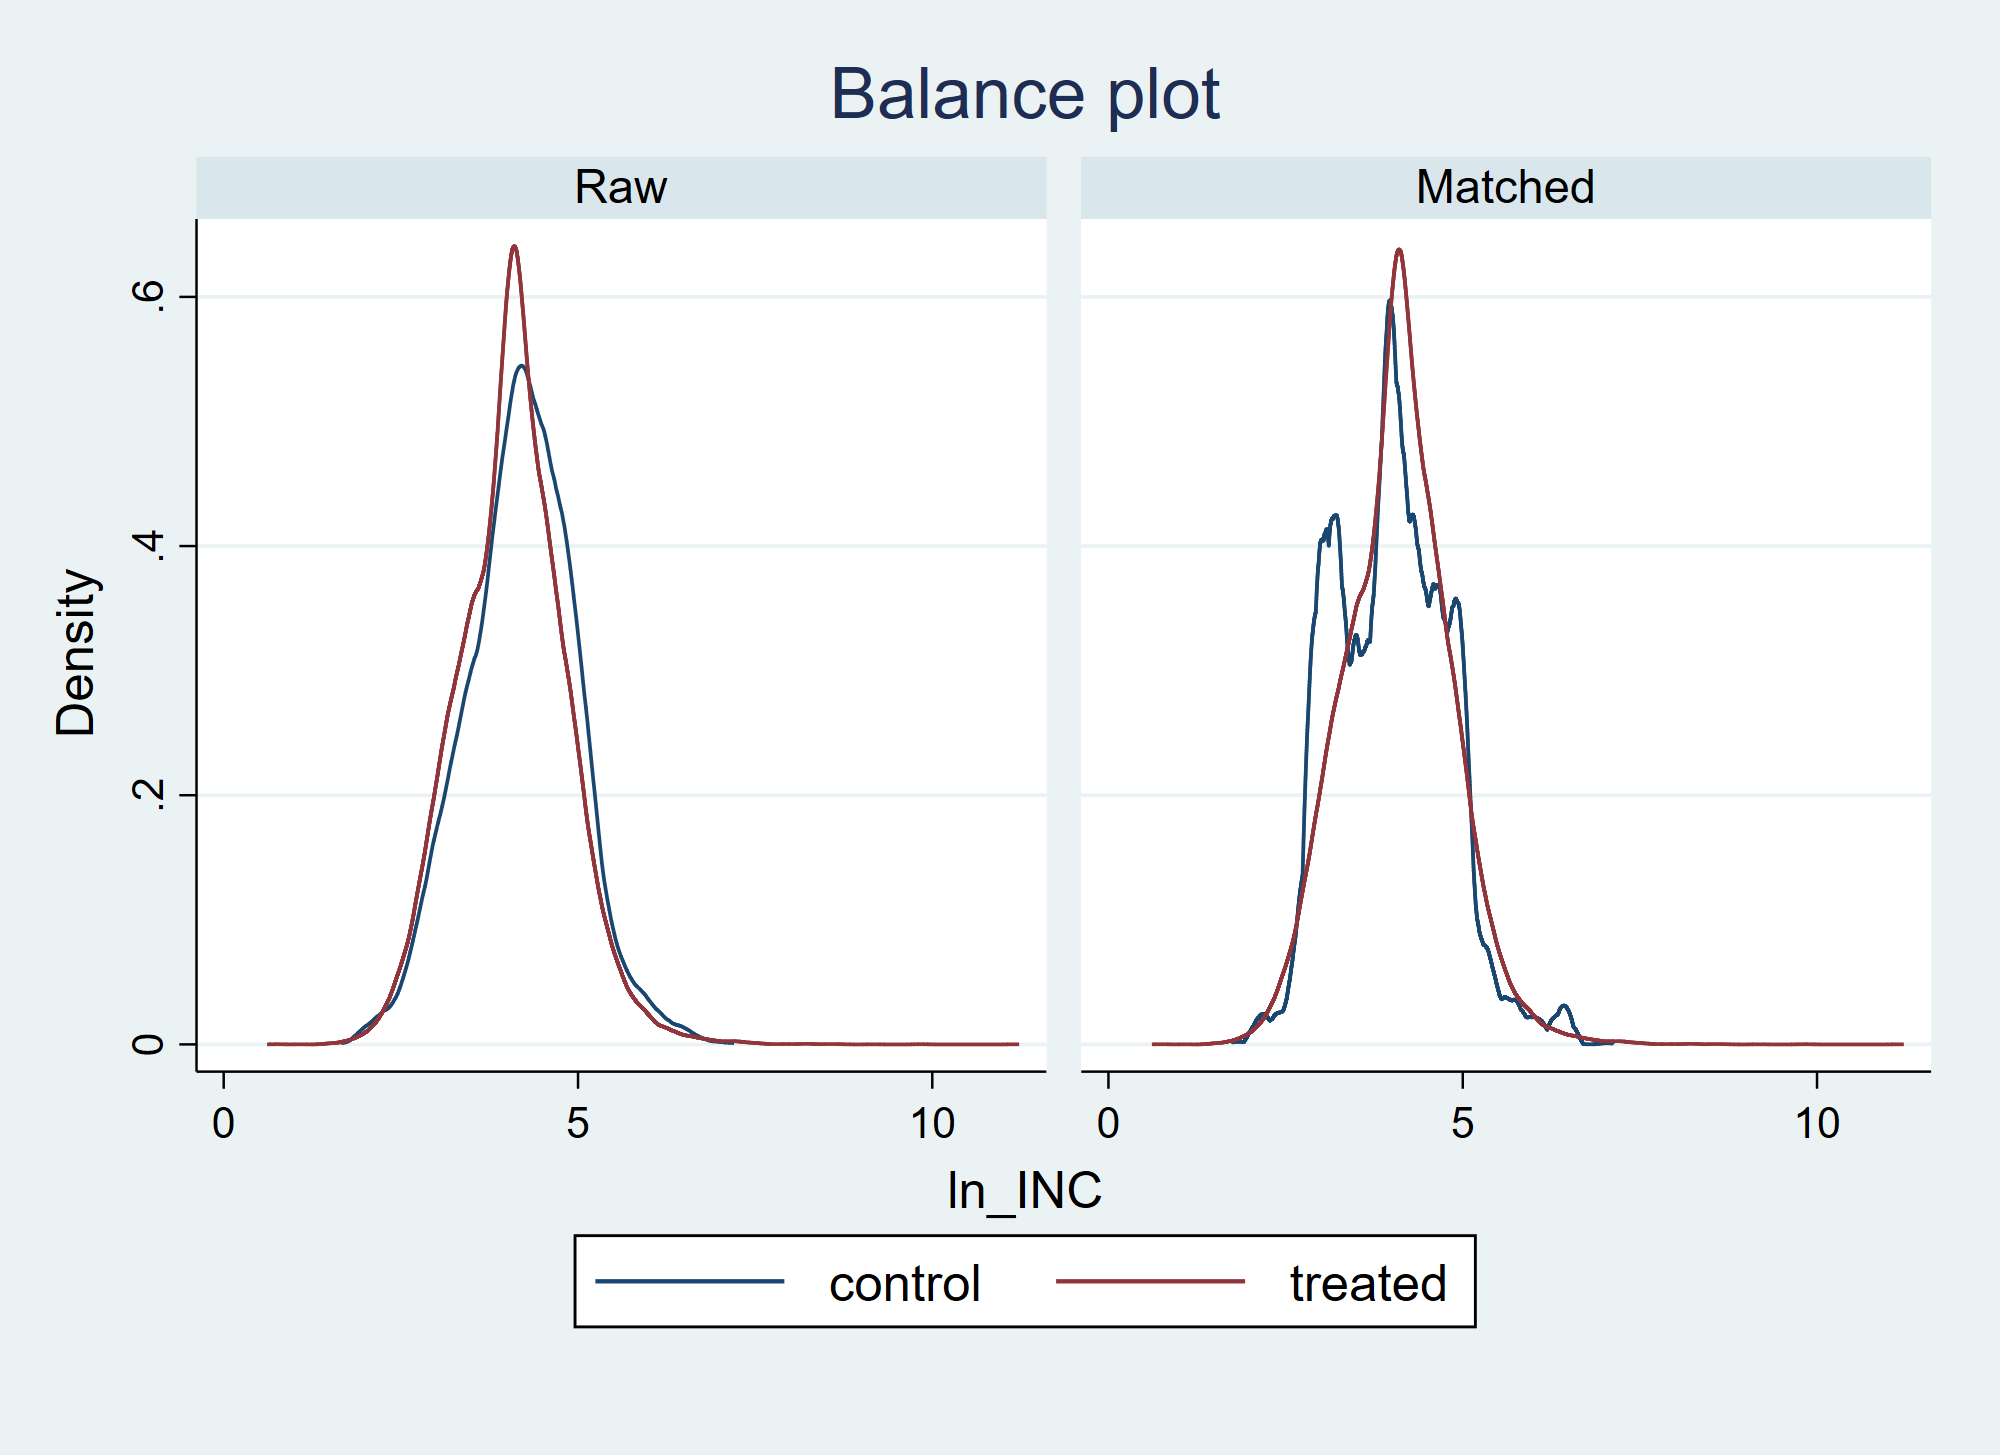
\includegraphics[width=0.8\textwidth]{figures/Figure3_Balance_Plot.png}
	\caption{Đánh giá chất lượng ghép cặp (Balance Plot) đối với biến Log Thu nhập}
	\label{fig:balance_plot}
\end{figure}

Để củng cố tính vững (robustness) của kết quả tổng, nghiên cứu áp dụng thuật toán Ghép cặp điểm xu hướng (PSM). Tác động ATE thu được là $+0.513$ ($p<0.001$), đồng thuận hoàn toàn với chiều hướng gia tăng chi phí của mô hình Total OOP (IV-2SLS). Đáng chú ý, Hình \ref{fig:balance_plot} minh chứng cho sự thành công của thuật toán: sau khi ghép cặp, hàm mật độ thu nhập của hai nhóm can thiệp và đối chứng đã trùng khớp gần như hoàn hảo, triệt tiêu hoàn toàn sự thiên lệch chọn mẫu do điều kiện kinh tế.

\subsubsection{Kết quả Ước lượng Biến Công Cụ (IV-2SLS)}

Để giải quyết vấn đề nội sinh của việc tham gia bảo hiểm y tế và các biến tương tác, nghiên cứu sử dụng phương pháp Hồi quy Biến công cụ Hai giai đoạn (IV-2SLS) với sai số chuẩn mạnh được san cụm (clustered) theo cấp tỉnh. Kết quả ước lượng ở giai đoạn 2 được trình bày trong Bảng \label{tab:iv_appendix} Phụ lục.

Kết quả cho thấy bảo hiểm y tế có tác động đáng kể đến chi tiêu y tế từ tiền túi (OOP) tính theo logarit. Cụ thể, tại mức cơ sở, việc có bảo hiểm y tế (\texttt{INS\_DUMMY}) làm tăng chi tiêu OOP một cách có ý nghĩa thống kê (hệ số ước lượng là $\mathbf{1.188}$, $p < 0.01$). Tuy nhiên, hiệu ứng này có sự khác biệt rõ rệt theo khu vực sinh sống. Biến tương tác giữa bảo hiểm y tế và khu vực nông thôn (\texttt{ins\_rural}) có hệ số âm và có ý nghĩa thống kê (hệ số $\mathbf{-1.147}$, $p < 0.01$). Điều này ngụ ý rằng, đối với người dân ở khu vực nông thôn, tác động làm tăng chi tiêu OOP của bảo hiểm y tế đã được triệt tiêu gần như hoàn toàn so với khu vực thành thị.

Về hành vi khám chữa bệnh vượt tuyến (\texttt{ins\_vuot}), kết quả chung không cho thấy tác động có ý nghĩa thống kê lên chi tiêu OOP ($p = 0.236$). Dẫu vậy, khi xét riêng nhóm có bảo hiểm y tế ở nông thôn có hành vi vượt tuyến (\texttt{ins\_rural\_vuot}), hệ số ước lượng mang dấu âm ($\mathbf{-3.318}$) và có ý nghĩa thống kê ở mức $10\%$ ($p = 0.096$), cho thấy dấu hiệu giảm chi tiêu OOP cho nhóm đối tượng cụ thể này. 

Mặc dù các kiểm định chẩn đoán ở giai đoạn 1 (trình bày chi tiết tại Phụ lục) cho thấy mô hình vượt qua kiểm định thiếu định dạng (Underidentification test), nhưng thống kê Kleibergen-Paap rk Wald F khá thấp ($\mathbf{2.77}$). Điều này cho thấy sự hiện diện của hiện tượng biến công cụ yếu (weak instruments) khi phải đồng thời xử lý 4 biến nội sinh. Do đó, các ước lượng ở giai đoạn 2 cần được diễn giải một cách thận trọng.

\subsection{Tổng hợp kết luận về kết quả định lượng}

Dựa trên chuỗi các phương pháp ước lượng và kiểm định tính vững, nghiên cứu rút ra những kết luận định lượng cốt lõi về tác động của bảo hiểm y tế (BHYT) đối với chi tiêu y tế từ tiền túi (OOP) như sau:

\begin{itemize}
	\item \textbf{Về độ tin cậy của mô hình:} Các chẩn đoán khuyết tật dữ liệu cho thấy mô hình tồn tại hiện tượng phương sai sai số thay đổi và tương quan nội cụm (hệ số ICC đạt mức $7.06\%$). Tuy nhiên, các vấn đề này đã được kiểm soát triệt để thông qua sai số chuẩn mạnh san cụm cấp tỉnh. Mô hình cũng được chứng minh là an toàn trước rủi ro đa cộng tuyến.
	
	\item \textbf{Tác động tổng thể của BHYT (Hiệu ứng mở rộng):} Cả mô hình Hồi quy Biến công cụ (IV-2SLS) và thuật toán Ghép cặp điểm xu hướng (PSM) đều cung cấp bằng chứng đồng nhất ở mức ý nghĩa $1\%$ ($p < 0.01$). Thay vì làm giảm chi tiêu, việc sở hữu thẻ BHYT lại làm tăng tổng chi phí OOP (mức tăng trung bình là $51.3\%$ theo ước lượng ATE của mô hình PSM). Kết quả này phản ánh rõ nét "hiệu ứng mở rộng" (moral hazard / expansion effect), trong đó BHYT gỡ bỏ rào cản tài chính ban đầu, kích thích người dân tiếp cận và sử dụng dịch vụ y tế với tần suất cao hơn, kéo theo sự gia tăng về khối lượng đồng chi trả.
	
	\item \textbf{Sự phân hóa tác động theo đặc điểm địa lý và hành vi:} Mô hình IV-2SLS chỉ ra sự dị biệt rõ rệt trong tác động của BHYT giữa các nhóm đối tượng:
	\begin{itemize}
		\item \textit{Yếu tố khu vực:} Đối với nhóm người có BHYT sinh sống tại nông thôn, tác động làm tăng chi phí OOP gần như được triệt tiêu hoàn toàn so với khu vực thành thị (hệ số tương tác là $-1.147$, $p < 0.01$).
		\item \textit{Yếu tố vượt tuyến:} Mặc dù hành vi khám vượt tuyến nói chung không tác động rõ rệt lên OOP ($p = 0.236$), nhưng đối với nhóm đặc thù là \textit{người có BHYT ở nông thôn thực hiện khám vượt tuyến}, chi tiêu OOP lại ghi nhận xu hướng giảm (hệ số $-3.318$, ý nghĩa ở mức $10\%$).
	\end{itemize}
	
	\item \textbf{Hạn chế về mặt thống kê:} Việc đồng thời công cụ hóa 4 biến nội sinh trong mô hình IV-2SLS đã dẫn đến hiện tượng biến công cụ yếu (thống kê Kleibergen-Paap rk Wald F chỉ đạt $2.77$). Do đó, các hệ số ước lượng trong IV-2SLS mang ý nghĩa chỉ báo về chiều hướng (dấu của tác động) nhiều hơn là mức độ chính xác tuyệt đối. Dẫu vậy, sự hỗ trợ chéo từ mô hình PSM (đã loại trừ thiên lệch chọn mẫu trên biến quan sát) đã bù đắp xuất sắc cho hạn chế này, khẳng định tính vững chắc của các phát hiện nghiên cứu.
\end{itemize}

\section{Kết luận và Hàm ý chính sách}

Nghiên cứu này bác bỏ quan điểm tuyến tính, một chiều cho rằng "Bảo hiểm y tế luôn làm giảm mọi loại chi phí từ tiền túi (OOP)". Bằng chứng nhân quả rút ra từ dữ liệu VHLSS 2024 chỉ ra rằng hệ thống BHYT tại Việt Nam đang vận hành theo một \textbf{"Hiệu ứng kép"}. Một mặt, BHYT đóng vai trò là chất xúc tác làm gia tăng chi phí y tế tổng thể do việc khai thông nhu cầu khám chữa bệnh bị kìm nén và sự hiện diện của rủi ro đạo đức (moral hazard). Mặt khác, nó lại phát huy trọn vẹn vai trò là "tấm khiên" bảo vệ tài chính, chặn đứng các cú sốc y tế thảm họa, đặc biệt là đối với nhóm bệnh nhân ở khu vực nông thôn khi buộc phải vượt tuyến để điều trị các bệnh lý nghiêm trọng.

Từ những phát hiện định lượng cốt lõi trên, nghiên cứu đề xuất ba hàm ý chính sách trọng tâm nhằm thúc đẩy lộ trình Bao phủ Y tế Phổ quát (SDG 3.8):

\begin{enumerate}
	\item \textbf{Đầu tư chiến lược cho mạng lưới y tế cơ sở tại nông thôn:} Mức gia tăng chi phí đột biến từ hành vi khám chữa bệnh vượt tuyến (hệ số $+2.038$ tại phân vị $Q90$) là một tín hiệu cảnh báo nghiêm trọng về năng lực đáp ứng của y tế tuyến dưới. Việc ưu tiên mở rộng danh mục thuốc được BHYT chi trả (đặc biệt là thuốc điều trị bệnh mãn tính) và nâng cao chất lượng dịch vụ tại các trạm y tế tuyến xã/huyện là giải pháp cấp bách. Giữ chân bệnh nhân tại cơ sở y tế ban đầu là cách thức bền vững nhất để triệt tiêu rủi ro "thảm họa kép" (gánh nặng chi phí điều trị cộng hưởng với chi phí phạt trái tuyến).
	
	\item \textbf{Đổi mới cơ chế thanh toán chi phí khám chữa bệnh:} Sự gia tăng chi phí có dấu hiệu bắt nguồn từ rủi ro đạo đức của cả phía cung (cơ sở y tế) và phía cầu (người bệnh). Hệ thống y tế cần đẩy nhanh tiến độ chuyển đổi từ phương thức thanh toán theo phí dịch vụ (Fee-for-service) sang thanh toán theo nhóm chẩn đoán (DRG - Diagnosis-Related Group) hoặc định suất (Capitation). Cơ chế thanh toán thông minh này sẽ triệt tiêu động cơ lạm dụng các chỉ định cận lâm sàng không cần thiết và hạn chế tình trạng kê đơn thuốc ngoài danh mục BHYT.
	
	\item \textbf{Duy trì và mở rộng lưới an sinh y tế cho nhóm yếu thế:} Hệ số tác động âm và lớn của BHYT khi đối phó với các cú sốc sức khỏe nặng là minh chứng rõ rệt nhất cho giá trị nhân đạo và tính ưu việt của hệ thống. Ngân sách Nhà nước cần tiếp tục ưu tiên phân bổ nhằm duy trì cơ chế hỗ trợ 100\% mức đóng BHYT cho người nghèo, cận nghèo và đồng bào dân tộc thiểu số tại khu vực nông thôn, đảm bảo nguyên tắc an sinh "không một ai bị bỏ lại phía sau" khi rủi ro bệnh tật ập đến.
\end{enumerate}

\section{Giới hạn của nghiên cứu và hướng phát triển} 
	
Việc thiếu vắng các biến số vi mô mô tả đặc tính phía cung (như khoảng cách vật lý chính xác từ hộ gia đình đến bệnh viện, hay mật độ bác sĩ trên vạn dân) trong bộ dữ liệu VHLSS là một hạn chế khách quan. Mặc dù nghiên cứu đã sử dụng các hiệu ứng cố định (Province FE) và biến công cụ (IV) để lọc bỏ sự nội sinh, các nghiên cứu trong tương lai nếu có thể liên kết (merge) dữ liệu khảo sát hộ gia đình với dữ liệu từ Hệ thống Thông tin Y tế Quốc gia (DHIS2) sẽ cung cấp một bức tranh toàn cảnh và chính xác hơn nữa về độ co giãn của cầu y tế theo không gian.


%====================================================
% APPENDIX 
%====================================================
\newpage
\appendix
\section{Phụ lục}

\subsection{Thống kê mô tả các biến số chính}

\begin{table}[htbp]
	\centering
	\caption{Thống kê mô tả các biến trong mô hình ($N = 46.995$)}
	\label{tab:summary_stats}
	\begin{tabular}{lcccc}
		\toprule
		\textbf{Biến số} & \textbf{Trung bình} & \textbf{Độ lệch chuẩn} & \textbf{Giá trị Min} & \textbf{Giá trị Max} \\
		\midrule
		\multicolumn{5}{l}{\textit{\textbf{Biến phụ thuộc (Chi phí y tế)}}} \\
		Tổng chi phí OOP (Triệu VND) & 5.578 & 13.040 & 0 & 660 \\
		Chi phí OOP Nội trú (Triệu VND) & 1.495 & 10.278 & 0 & 600 \\
		Chi phí OOP Ngoại trú (Triệu VND) & 1.341 & 5.141 & 0 & 324 \\
		\addlinespace
		\multicolumn{5}{l}{\textit{\textbf{Biến độc lập chính và Đặc điểm hộ gia đình}}} \\
		Bảo hiểm y tế ($INS\_DUMMY$: 1=Có) & 0.971 & 0.168 & 0 & 1 \\
		Hành vi vượt tuyến ($BYPASSED$: 1=Có) & 0.375 & 0.484 & 0 & 1 \\
		Khu vực Nông thôn ($RURAL$: 1=Có) & 0.603 & 0.489 & 0 & 1 \\
		Log thu nhập bình quân ($\ln\_INC$) & 4.162 & 0.752 & 0.697 & 11.149 \\
		Tuổi chủ hộ ($AGE\_HEAD$) & 53.945 & 13.675 & 10 & 106 \\
		Giới tính chủ hộ ($SEX\_HEAD$: 1=Nam) & 0.700 & 0.458 & 0 & 1 \\
		Quy mô hộ gia đình ($HH\_SIZE$) & 3.513 & 1.646 & 1 & 16 \\
		\addlinespace
		\multicolumn{5}{l}{\textit{\textbf{Biến công cụ (Instrumental Variable)}}} \\
		Tỷ lệ BHYT cấp xã ($IV\_COMMUNE$) & 0.925 & 0.100 & 0.026 & 1 \\
		\bottomrule
	\end{tabular}
	\vspace{0.15cm}
	
	\parbox{14cm}{\footnotesize \textit{Ghi chú:} Thống kê mô tả đã áp dụng trọng số mẫu (sample weights) của VHLSS 2024. Trung bình tỷ lệ BHYT ($INS\_DUMMY$) đạt 97,08\% (làm tròn thành 0.971). Biến giới tính chủ hộ đã được chuẩn hóa về dạng Dummy (0=Nữ, 1=Nam).}
\end{table}

\newpage
\subsection{Kết quả định lượng chi tiết}
\subsubsection{Phụ lục A – Kết quả mô hình biến công cụ (IV-2SLS phân rã OOP)}

\begin{table}[htbp]
	\centering
	\def\sym#1{\ifmmode^{#1}\else\(^{#1}\)\fi}
	\caption{Tác động của BHYT lên cấu trúc chi phí OOP (Mô hình IV-2SLS)}
	\label{tab:iv_appendix}
	\begin{tabular}{lccc}
		\toprule
		&\textbf{(1)}&\textbf{(2)}&\textbf{(3)}\\
		\textbf{Biến độc lập}&\textbf{Log(Tổng OOP)}&\textbf{Log(OOP Nội trú)}&\textbf{Log(OOP Ngoại trú)}\\
		\midrule
		BHYT (Cơ sở) & 1.256\sym{***} & -0.219 & 0.292\sym{*} \\
		& (0.177) & (0.155) & (0.157) \\
		\addlinespace
		BHYT $\times$ Nông thôn & -0.967\sym{***} & -0.115 & 0.035 \\
		& (0.286) & (0.178) & (0.137) \\
		\addlinespace
		BHYT $\times$ Vượt tuyến & 2.413 & 2.806 & 0.405 \\
		& (1.833) & (2.172) & (1.513) \\
		\addlinespace
		BHYT $\times$ Nông thôn $\times$ Vượt tuyến & -3.533 & -1.345 & -2.971\sym{*} \\
		& (2.151) & (2.431) & (1.707) \\
		\addlinespace
		Nông thôn (Base) & 0.850\sym{***} & 0.083 & -0.026 \\
		& (0.262) & (0.155) & (0.133) \\
		\addlinespace
		Vượt tuyến (Base) & -1.648 & -2.244 & 0.443 \\
		& (1.795) & (2.092) & (1.493) \\
		\midrule
		Biến kiểm soát ($X$) & Có & Có & Có \\
		Fixed Effects (Tỉnh) & Có & Có & Có \\
		\midrule
		Số quan sát ($N$) & 46.995 & 46.995 & 46.995 \\
		\bottomrule
		\multicolumn{4}{p{13cm}}{\footnotesize \textit{Ghi chú:} Sai số chuẩn vững (Robust standard errors) được cụm theo cấp tỉnh đặt trong ngoặc đơn. \newline \sym{*} \(p<0.10\), \sym{**} \(p<0.05\), \sym{***} \(p<0.01\)}
	\end{tabular}
\end{table}

\newpage
\subsubsection{Phụ lục B – Kết quả hồi quy Phân vị đồng thời (SQREG)}

\begin{table}[htbp]
	\centering
	\def\sym#1{\ifmmode^{#1}\else\(^{#1}\)\fi}
	\caption{Tác động của BHYT dọc theo phân phối chi phí (Mô hình SQREG)}
	\label{tab:sqreg_appendix}
	\begin{tabular}{lcccc}
		\toprule
		&\textbf{(1)}&\textbf{(2)}&\textbf{(3)}&\textbf{(4)}\\
		\textbf{Biến độc lập}&\textbf{Q25}&\textbf{Q50}&\textbf{Q75}&\textbf{Q90}\\
		\midrule
		BHYT (Cơ sở) & 0.585\sym{***} & 0.681\sym{***} & 0.669\sym{***} & 0.675\sym{***} \\
		& (0.025) & (0.023) & (0.033) & (0.043) \\
		\addlinespace
		Vượt tuyến & 0.558\sym{***} & 0.916\sym{***} & 1.654\sym{***} & 2.039\sym{***} \\
		& (0.081) & (0.088) & (0.121) & (0.228) \\
		\addlinespace
		BHYT $\times$ Nông thôn & -0.198\sym{***} & -0.073\sym{***} & 0.014 & -0.011 \\
		& (0.030) & (0.024) & (0.041) & (0.064) \\
		\addlinespace
		BHYT $\times$ Vượt tuyến & -0.045 & -0.290\sym{***} & -0.643\sym{***} & -0.605\sym{***} \\
		& (0.083) & (0.090) & (0.125) & (0.228) \\
		\addlinespace
		BHYT $\times$ Nông thôn $\times$ Vượt tuyến & 0.170\sym{***} & 0.079\sym{***} & 0.055\sym{**} & 0.044 \\
		& (0.019) & (0.017) & (0.025) & (0.031) \\
		\addlinespace
		Log(Thu nhập) & 0.267\sym{***} & 0.204\sym{***} & 0.154\sym{***} & 0.168\sym{***} \\
		& (0.005) & (0.005) & (0.006) & (0.007) \\
		\midrule
		Biến kiểm soát nhân khẩu học & Có & Có & Có & Có \\
		\midrule
		Pseudo $R^2$ & 0.202 & 0.209 & 0.260 & 0.314 \\
		Số quan sát ($N$) & 46.995 & 46.995 & 46.995 & 46.995 \\
		\bottomrule
		\multicolumn{5}{p{13.5cm}}{\footnotesize \textit{Ghi chú:} Mô hình Hồi quy phân vị đồng thời (Simultaneous Quantile Regression) với 100 lần bootstrap để tính sai số chuẩn (đặt trong ngoặc đơn). Biến giả kiểm soát cấp tỉnh (Province FE) được loại bỏ để đảm bảo sự hội tụ của mô hình ở các phân vị biên. \newline \sym{*} \(p<0.10\), \sym{**} \(p<0.05\), \sym{***} \(p<0.01\)}
	\end{tabular}
\end{table}

\newpage
\subsubsection{Phụ lục C – Kết quả Ghép cặp điểm xu hướng (PSM)}

\begin{table}[htbp]
	\centering
	\def\sym#1{\ifmmode^{#1}\else\(^{#1}\)\fi}
	\caption{Kết quả đánh giá tác động BHYT bằng thuật toán ghép cặp NNM 1-1}
	\label{tab:psm_appendix}
	\begin{tabular}{lc}
		\toprule
		\textbf{Chỉ số đánh giá} & \textbf{Log(Tổng OOP)} \\
		\midrule
		\textbf{Tác động xử lý trung bình (ATE)} & \textbf{0.513\sym{***}} \\
		& (0.082) \\
		\addlinespace
		Giá trị thống kê ($z$-statistic) & 6.19 \\
		Giá trị $p$ ($p$-value) & 0.000 \\
		Khoảng tin cậy 95\% (95\% CI) & [0.350, 0.675] \\
		\midrule
		Số quan sát được ghép cặp ($N$) & 46.744 \\
		\bottomrule
		\multicolumn{2}{p{11.5cm}}{\footnotesize \textit{Ghi chú:} Mô hình Probit được sử dụng để ước lượng điểm xu hướng. Tác động của BHYT được so sánh giữa nhóm có thẻ ($1$) và không có thẻ ($0$). Các quan sát vi phạm Vùng hỗ trợ chung (Common Support) đã được loại bỏ trước khi ghép cặp nhằm giảm thiểu chệch lựa chọn. Sai số chuẩn AI (Abadie-Imbens robust standard errors) đặt trong ngoặc đơn. \newline \sym{***} \(p<0.01\)} \\
	\end{tabular}
\end{table}

\newpage
\subsubsection{Phụ lục D - Kiểm định Đa cộng tuyến (VIF)}

\begin{table}[htbp]
	\centering
	\caption{Kết quả kiểm định VIF cho mô hình cơ sở}
	\label{tab:vif_test}
	\begin{tabular}{lcc}
		\toprule
		\textbf{Biến số} & \textbf{VIF} & \textbf{1/VIF} \\
		\midrule
		\textbf{Các biến chính và biến tương tác} & & \\
		\texttt{INS\_DUMMY} & 2.48 & 0.403 \\
		\texttt{RURAL} & 32.70 & 0.031 \\
		\texttt{hh\_vuot\_tuyen} & 72.65 & 0.014 \\
		\texttt{ins\_rural} & 34.60 & 0.029 \\
		\texttt{ins\_vuot} & 74.88 & 0.013 \\
		\texttt{ins\_rural\_vuot} & 3.07 & 0.326 \\
		\midrule
		\textbf{Các biến kiểm soát (X)} & & \\
		\texttt{ln\_INC} & 1.23 & 0.812 \\
		\texttt{AGE\_HEAD} & 1.15 & 0.869 \\
		\texttt{HH\_SIZE} & 1.15 & 0.868 \\
		\texttt{SEX\_HEAD} & 1.10 & 0.912 \\
		\midrule
		\textbf{Mean VIF} & \multicolumn{2}{c}{\textbf{4.14}} \\
		\bottomrule
	\end{tabular}
	
	\vspace{1ex}
	\raggedright \textit{\small Ghi chú: Các biến giả kiểm soát hiệu ứng cố định cấp tỉnh (\texttt{i.tinh}) đã được đưa vào mô hình nhưng không trình bày chi tiết trong bảng này để tiết kiệm không gian. Giá trị VIF của toàn bộ các biến giả cấp tỉnh đều dao động ở mức rất thấp (từ 1.05 đến 2.21).}
\end{table}

\newpage
\subsubsection{Phụ lục E - Ma trận tương quan (Correlation Matrix)}

\begin{table}[htbp]
	\centering
	\caption{Ma trận tương quan có trọng số giữa các biến trong mô hình}
	\label{tab:corr_matrix}
	\resizebox{\textwidth}{!}{% Thu nhỏ bảng vừa với chiều rộng trang giấy
		\begin{tabular}{lccccccccccc}
			\toprule
			\textbf{Biến số} & \textbf{(1)} & \textbf{(2)} & \textbf{(3)} & \textbf{(4)} & \textbf{(5)} & \textbf{(6)} & \textbf{(7)} & \textbf{(8)} & \textbf{(9)} & \textbf{(10)} & \textbf{(11)} \\
			\midrule
			(1) \texttt{ln\_OOP} & 1.000 & & & & & & & & & & \\
			(2) \texttt{INS\_DUMMY} & 0.187 & 1.000 & & & & & & & & & \\
			(3) \texttt{RURAL} & -0.063 & 0.016 & 1.000 & & & & & & & & \\
			(4) \texttt{hh\_vuot\_tuyen} & 0.509 & 0.092 & -0.078 & 1.000 & & & & & & & \\
			(5) \texttt{ins\_rural} & -0.027 & 0.210 & 0.966 & -0.060 & 1.000 & & & & & & \\
			(6) \texttt{ins\_vuot} & 0.509 & 0.135 & -0.078 & 0.992 & -0.051 & 1.000 & & & & & \\
			(7) \texttt{ins\_rural\_vuot} & 0.347 & 0.090 & 0.413 & 0.656 & 0.428 & 0.661 & 1.000 & & & & \\
			(8) \texttt{ln\_INC} & 0.129 & -0.029 & -0.264 & 0.001 & -0.261 & -0.000 & -0.120 & 1.000 & & & \\
			(9) \texttt{AGE\_HEAD} & 0.094 & 0.038 & 0.028 & 0.153 & 0.033 & 0.155 & 0.116 & -0.125 & 1.000 & & \\
			(10) \texttt{SEX\_HEAD} & 0.059 & 0.015 & 0.125 & -0.029 & 0.124 & -0.028 & 0.050 & 0.014 & -0.143 & 1.000 & \\
			(11) \texttt{HH\_SIZE} & 0.284 & 0.141 & 0.049 & 0.055 & 0.074 & 0.060 & 0.059 & -0.139 & -0.141 & 0.214 & 1.000 \\
			\bottomrule
		\end{tabular}%
	}
	
	\vspace{1ex}
	\raggedright \textit{\small Ghi chú: Kích thước mẫu quan sát $N = 46,995$. Do cỡ mẫu rất lớn, hầu hết các hệ số tương quan đều có ý nghĩa thống kê ở mức $1\%$ ($p < 0.01$). Các hệ số tương quan rất cao (như giữa \texttt{RURAL} và \texttt{ins\_rural} là $0.966$, hoặc \texttt{hh\_vuot\_tuyen} và \texttt{ins\_vuot} là $0.992$) là hệ quả tất yếu do đây là cấu trúc của các biến tương tác (interaction terms), điều này hoàn toàn phù hợp với lý thuyết toán học và lý giải cho kết quả kiểm định VIF cao tại các biến này ở Phụ lục trước.}
\end{table}

\newpage
\subsubsection{Phụ lục F – Kiểm định Chẩn đoán Hồi quy Giai đoạn 1 (First-Stage Diagnostics cho Mô hình IV-2SLS)}

Bảng dưới đây tóm tắt các kết quả kiểm định chẩn đoán tính hợp lệ và sức mạnh của 4 biến công cụ loại trừ (\texttt{IV\_COMMUNE}, \texttt{iv\_rural}, \texttt{iv\_vuot}, \texttt{iv\_rural\_vuot}) đối với 4 biến nội sinh (\texttt{INS\_DUMMY}, \texttt{ins\_rural}, \texttt{ins\_vuot}, \texttt{ins\_rural\_vuot}). Số liệu quan sát là $46,995$ và sai số được san cụm theo $63$ tỉnh/thành.

\begin{table}[htbp]
	\centering
	\caption{Thống kê F-test ở giai đoạn 1 cho từng biến nội sinh}
	\label{tab:first_stage_f_tests}
	\begin{tabular}{lcccc}
		\toprule
		\textbf{Biến nội sinh} & \textbf{F-test (truyền thống)} & \textbf{p-value} & \textbf{SW F-test} & \textbf{p-value} \\
		\midrule
		\texttt{INS\_DUMMY} & 96.68 & 0.000 & 96.65 & 0.000 \\
		\texttt{ins\_rural} & 90.66 & 0.000 & 418.55 & 0.000 \\
		\texttt{ins\_vuot} & 9.72 & 0.000 & 172.15 & 0.000 \\
		\texttt{ins\_rural\_vuot} & 15.64 & 0.000 & 534.43 & 0.000 \\
		\bottomrule
	\end{tabular}
	
	\vspace{1ex}
	\raggedright \textit{\small Ghi chú: Thống kê SW F-test (Sanderson-Windmeijer) đánh giá sức mạnh độc lập của biến công cụ đối với từng biến nội sinh riêng biệt sau khi đã loại bỏ ảnh hưởng của các biến nội sinh khác.}
\end{table}


\newpage
\subsubsection{Phụ lục G – Kết quả kiểm định khuyết tật của mô hình}
	
	\begin{table}[htbp]
		\centering
		\caption{Kết quả kiểm định khuyết tật của mô hình (Mô hình IV-2SLS)}
		\label{tab:diagnostics}
		\begin{tabular}{llcc}
			\toprule
			\textbf{Loại kiểm định} & \textbf{Thống kê / Hệ số} & \textbf{Giá trị} & \textbf{P-value} \\
			\midrule
			\multicolumn{4}{l}{\textbf{Panel A: Kiểm định phương sai sai số thay đổi}} \\
			Kiểm định Pagan-Hall & Thống kê $\chi^2(8)$ & 2982.260 & 0.0000 \\
			\textit{($H_0$: Phương sai sai số đồng nhất)} & & & \\
			\midrule
			\multicolumn{4}{l}{\textbf{Panel B: Kiểm định tương quan nội cụm theo Tỉnh}} \\
			Phân tích ANOVA một chiều & Thống kê $F(62, 46932)$ & 57.50 & 0.0000 \\
			\textit{($H_0$: Không có hiệu ứng cấp tỉnh)} & & & \\
			\addlinespace
			Hệ số tương quan nội cụm & Giá trị ICC & 0.0706 & - \\
			& Sai số chuẩn (Asy. S.E.) & (0.0127) & \\
			& Khoảng tin cậy 95\% & [0.0457, 0.0954] & \\
			\bottomrule
		\end{tabular}
		
		\vspace{1ex}
		\raggedright \textit{\small Ghi chú: Kích thước mẫu $N = 46,995$. Ở Panel A, kiểm định Pagan-Hall được sử dụng thay cho Breusch-Pagan do tính phù hợp với mô hình có chứa biến công cụ (IV). Với $p < 0.01$, giả thuyết $H_0$ bị bác bỏ, khẳng định sự tồn tại của phương sai sai số thay đổi. Ở Panel B, hệ số ICC cho thấy khoảng 7.06\% phương sai của biến phụ thuộc được cấu thành từ các đặc điểm không quan sát được ở cấp tỉnh, đồng thời thống kê F có ý nghĩa ở mức 1\%, xác nhận hiện tượng tự tương quan không gian nội cụm.}
	\end{table}
	
%====================================================
% REFERENCES
%====================================================
\newpage
\section*{Tài liệu tham khảo}
\addcontentsline{toc}{section}{Tài liệu tham khảo}
\printbibliography[heading=none, title={}]
\renewcommand{\bibfont}{\small}

\end{document}